%%%%%%%%%%%%%%%%%%%% book.tex %%%%%%%%%%%%%%%%%%%%%%%%%%%%%
%
% sample root file for the chapters of your "monograph"
%
% Use this file as a template for your own input.
%
%%%%%%%%%%%%%%%% Springer-Verlag %%%%%%%%%%%%%%%%%%%%%%%%%%


% RECOMMENDED %%%%%%%%%%%%%%%%%%%%%%%%%%%%%%%%%%%%%%%%%%%%%%%%%%%
\documentclass[graybox,envcountchap,sectrefs]{svmono}

% choose options for [] as required from the list
% in the Reference Guide

%\usepackage{mathptmx}
%\usepackage{helvet}
%\usepackage{courier}
%
\usepackage{type1cm}         

\usepackage{makeidx}         % allows index generation
\usepackage{graphicx}        % standard LaTeX graphics tool
                             % when including figure files
\usepackage{multicol}        % used for the two-column index
\usepackage[bottom]{footmisc}% places footnotes at page bottom

\usepackage{newtxtext}       % 
\usepackage{newtxmath}       % selects Times Roman as basic font
\usepackage{empheq}
\usepackage[most]{tcolorbox}
\usepackage{calc}
\usepackage{tikz}
\usepackage{hyperref}



% \newtcbox{\mybox}[1][]{%
%     nobeforeafter, math upper, tcbox raise base,
%     enhanced, colframe=blue!30!black,
%     colback=blue!30, boxrule=1pt,
%     #1}

%custom packages
%Simple shortcut commands
\newcommand{\pint}[3]{\int_{#1} \left( #2 \right) d#3}
\newcommand{\sint}[3]{\int_{#1} #2 \hspace{3pt} d#3}
\newcommand{\bs}[1]{\boldsymbol{#1}}
\newcommand{\pd}[2]{\frac{\partial #1}{\partial #2}}
\newcommand{\mc}[1]{\mathcal{#1}}
\newcommand{\tu}[1]{\textup{#1}}
\newcommand{\mbb}[1]{\mathbb{#1}}
\newcommand{\argmin}[1]{\underset{#1}{\textup{arg min }}}
\newcommand{\tbf}[1]{\textbf{#1}}
\newcommand{\tbfr}[1]{\textbf{\textcolor{red}{#1}}}
\newcommand{\R}{\mathbb{R}}
\newcommand{\PR}{\mathbb{P}}
\newcommand{\N}{\mathbb{N}}
%\newcommand{\E}{\mathbb{E}}
\newcommand{\EE}[1]{\mathbb{E}\left[#1\right]}
\newcommand{\indprob}[1]{\mathds{1}_{\left\{#1\right\}}}
\newcommand{\inwedge}[1]{\langle #1 \rangle}
\newcommand{\ncc}[4]{\textcolor{#1}{#3}\textcolor{#2}{#4}}
\newcommand{\nccc}[6]{\ncc{#1}{#2}{#4}{#5}\textcolor{#3}{#6}}
\newcommand{\ncccc}[8]{\ncc{#1}{#2}{#5}{#6}\ncc{#3}{#4}{#7}{#8}}
\newcommand{\tc}[2]{\textcolor{#1}{#2}}
\newcommand{\tcr}[1]{\textcolor{red}{#1}}
\newcommand{\tcc}[1]{\texcolor{violet}{#1}}
\newcommand{\q}[1]{``#1''}
\newcommand{\bt}[1]{\textbf{#1}}
\newcommand{\txt}[1]{\textup{#1}}
\newcommand{\pref}[1]{(\ref{#1})}

\newcommand\subt[1]{%
  \pgfmathparse{#1-1}\pgfmathresult%
}

\newcommand{\cbeqn}[2]{
\begin{empheq}[box=\tcbhighmath]{gather}
 \textbf{#1} \nonumber \\
 #2
\end{empheq}
}

\newcommand{\bjorn}{Bj\"{o}rn}
\newcommand{\askbjorn}[1]{\textcolor{red}{Ask \bjorn: #1}}

%More complicated commands found on Internet
\newcommand*\widefbox[1]{\fbox{\hspace{2em}#1\hspace{2em}}}
\newcommand{\rpm}{\sbox0{$1$}\sbox2{$\scriptstyle\pm$}
  \raise\dimexpr(\ht0-\ht2)/2\relax\box2 }
 
%Custom environments
\newenvironment{ceqn}
    {\begin{equation}
    \begin{aligned}
    }
    { 
    \end{aligned} 
    \end{equation}
    }
    


% see the list of further useful packages
% in the Reference Guide

\makeindex             % used for the subject index
                       % please use the style svind.ist with
                       % your makeindex program

%%%%%%%%%%%%%%%%%%%%%%%%%%%%%%%%%%%%%%%%%%%%%%%%%%%%%%%%%%%%%%%%%%%%%

\graphicspath{{./}{images/}}

\begin{document}

\author{Bj\"{o}rn Engquist \and Tyler Masthay}
\title{Mathematical Modeling}
%\subtitle{-- Monograph --}
\maketitle

\frontmatter%%%%%%%%%%%%%%%%%%%%%%%%%%%%%%%%%%%%%%%%%%%%%%%%%%%%%%

%
%%%%%%%%%%%%%%%%%%%%%%% dedic.tex %%%%%%%%%%%%%%%%%%%%%%%%%%%%%%%%%
%
% sample dedication
%
% Use this file as a template for your own input.
%
%%%%%%%%%%%%%%%%%%%%%%%% Springer %%%%%%%%%%%%%%%%%%%%%%%%%%

\begin{dedication}
\end{dedication}





%%%%%%%%%%%%%%%%%%%%%%%foreword.tex%%%%%%%%%%%%%%%%%%%%%%%%%%%%%%%%%
% sample foreword
%
% Use this file as a template for your own input.
%
%%%%%%%%%%%%%%%%%%%%%%%% Springer %%%%%%%%%%%%%%%%%%%%%%%%%%

\foreword

%% Please have the foreword written here
If we want a foreward, then we probably talk about the history of mathematical modeling. Similar to how Tinsley Oden goes all the way back to ancient Greeks at the start of his talks.



%%%%%%%%%%%%%%%%%%%%%%preface.tex%%%%%%%%%%%%%%%%%%%%%%%%%%%%%%%%%%%%%%%%%
% sample preface
%
% Use this file as a template for your own input.
%
%%%%%%%%%%%%%%%%%%%%%%%% Springer %%%%%%%%%%%%%%%%%%%%%%%%%%

\preface

This set of lecture notes is intended to supplement the courses \textit{Introduction to Mathematical Modeling I and II} taught during the first year of the CSEM program at UT-Austin. While these courses are focused mainly on physics, this course surveys mathematical modeling more generally. We will investigate problems that do not necessitate physics to model, e.g. traffic flow. We will also investigate data-driven models, e.g. models obtained through artificial neural networks. There are no formal requirements but background in differential equations, scientific programming and some probability will be useful. \tc{red}{Cross check with Bj\"{o}rn}.
 

\vspace{\baselineskip}
\begin{flushright}\noindent
\hfill {\it Bj\"{o}rn Engquist}\\
\hfill {\it Tyler Masthay}\\
\end{flushright}



%%%%%%%%%%%%%%%%%%%%%%%acknow.tex%%%%%%%%%%%%%%%%%%%%%%%%%%%%%%%%%%%%%%%%%
% sample acknowledgement chapter
%
% Use this file as a template for your own input.
%
%%%%%%%%%%%%%%%%%%%%%%%% Springer %%%%%%%%%%%%%%%%%%%%%%%%%%

\extrachap{Acknowledgements}

Use the template \emph{acknow.tex} together with the document class SVMono (monograph-type books) or SVMult (edited books) if you prefer to set your acknowledgement section as a separate chapter instead of including it as last part of your preface.



\tableofcontents

%%%%%%%%%%%%%%%%%%%%%%acronym.tex%%%%%%%%%%%%%%%%%%%%%%%%%%%%%%%%%%%%%%%%%
% sample list of acronyms
%
% Use this file as a template for your own input.
%
%%%%%%%%%%%%%%%%%%%%%%%% Springer %%%%%%%%%%%%%%%%%%%%%%%%%%

\extrachap{Acronyms}

\begin{description}[CABR]
\item[ANN]{Artificial Neural Network}
\item[SGD]{Stochastic Gradient Descent}
\item[POD]{Proper Orthogonal Decomposition}
\item[BVP]{Boundary-value problem}
\end{description}


\mainmatter%%%%%%%%%%%%%%%%%%%%%%%%%%%%%%%%%%%%%%%%%%%%%%%%%%%%%%%
%%%%%%%%%%%%%%%%%%%%%part.tex%%%%%%%%%%%%%%%%%%%%%%%%%%%%%%%%%%
% 
% sample part title
%
% Use this file as a template for your own input.
%
%%%%%%%%%%%%%%%%%%%%%%%% Springer %%%%%%%%%%%%%%%%%%%%%%%%%%

\begin{partbacktext}
\part{Part Title}
\noindent Use the template \emph{part.tex} together with the document class SVMono (monograph-type books) or SVMult (edited books) to style your part title page and, if desired, a short introductory text (maximum one page) on its verso page.

\end{partbacktext}
%%%%%%%%%%%%%%%%%%%%% chapter.tex %%%%%%%%%%%%%%%%%%%%%%%%%%%%%%%%%
%
% sample chapter
%
% Use this file as a template for your own input.
%
%%%%%%%%%%%%%%%%%%%%%%%% Springer-Verlag %%%%%%%%%%%%%%%%%%%%%%%%%%
%\motto{Use the template \emph{chapter.tex} to style the various elements of your chapter content.}
\chapter{Lecture 1: Course Outline and Toy Model}
\date{January 19, 2022}
\label{intro} % Always give a unique label
% use \chaptermark{}
% to alter or adjust the chapter heading in the running head

%\abstract*{Each chapter should be preceded by an abstract (no more than 200 words) that summarizes the content. The abstract will appear \textit{online} at \url{www.SpringerLink.com} and be available with unrestricted access. This allows unregistered users to read the abstract as a teaser for the complete chapter.
%Please use the 'starred' version of the new \texttt{abstract} command for typesetting the text of the online abstracts (cf. source file of this chapter template \texttt{abstract}) and include them with the source files of your manuscript. Use the plain \texttt{abstract} command if the abstract is also to appear in the printed version of the book.}

\abstract{We outline the course objectives and topics. We will analyze a toy model for the spread of infectious disease and of traffic flow.}

\section{Course Outline}
\label{sec:1}
In this course, we will focus on basic principles of mathematical modeling in contrast to courses that concentrate on methods tailored to specific classes of applications. \tc{red}{Reword slide ending in social sciences and finance}

\section{The Modeling Process}
Broadly speaking, the modeling process falls into three categories: \bt{physics-based modeling}, \bt{data-driven modeling}, and \bt{model reduction}. In our context, a \q{physics-based model} is meant to encompass a larger space of models than one would typically apply the term \q{physics} to. \tcr{By physics-based model, we mean...cause and effect is not a great description...skip data driven approach for now also}. Model reduction involves the generation of a less complex model from a more complex model. For example, if our model is given by a matrix $A \in \R^{n\times n}$, we can reduce this model to a matrix $B \in \R^{r \times r}$ to be the best rank $r$ approximation of $A$, i.e. the truncated SVD of $A$ of order $r$. 

\subsection{Physics-based Modeling}
\tcr{Let us come back to this whole section for later.}

\section{Relevant Properties of the Mathematical Model}
The three main properties we will discuss are well-posedness (model must make sense), complexity (model should not be overly complicated), and model-data interaction (model and data must match).
\subsection{Well-posedness}
Well-posedness consists of three classical conditions that must be satisfied. These are (a) existence of a solution for all model parameters, (b) uniqueness, i.e. that there exists one and only solution for any given model parameter, and (c) continuous dependence on data, i.e. small perturbations in parameter space lead to small perturbations in output space. If conditions (a), (b), and (c) hold, then our model is as well-behaved as we would reasonably expect. In practice, we may have one of these conditions not hold. 
\subsubsection{Existence}
Lack of existence is possibly the worst condition to not have satisfied. An example of this may occur when we have an overdetermined system, as can be the case for a passive advection model where concentrations are measured at both inflow and outflow.
\subsubsection{Uniqueness}
Uniqueness is necessary to be able to assess model quality, in some sense. Let us define our model as a relation $M \subseteq A \times B$ for parameter space $A$ and output space $B$. Uniqueness says that $M$ is, in fact, a function. That is,
\begin{align*}
    (a,b_1) \in M \txt{ and } (a,b_2) \in M \Rightarrow b_1 = b_2
\end{align*} 
Nonuniqueness is to say that $M$ is not a function. This intutively means that our model is poor.
\subsubsection{Continuous Dependence on Data}
\q{Data} in this context really means \q{parameter space}. For example, these could be initial conditions, physical parameters such as diffusivity of a chemical species, variance of noisy input to a stochastic differential equation, hyperparameters for a neural network, etc. Given that we cannot \q{see} all of parameter space, we would like small perturbations in parameter space to lead to only small perturbations in output space. Consider a model $F:(P,\|\cdot\|_P) \to (O, \|\cdot\|_{O})$ defined on normed vector spaces. We say that $F$ \textit{ depends continuously on data } if and only if for any sequences of parameters $p_{n}$,
\begin{align} \label{1:cdd}
    p_n \overset{P}{\to} p \Rightarrow F(p_n) \overset{O}{\to} F(p).
\end{align}
For example, consider $F:(\R^{n}, \|\cdot\|_{2}) \to (\R^{n}, \|\cdot\|_{2})$ by 
\begin{align}\label{1:matinv}
    F(\bs{b}) = \bs{x} \Leftrightarrow A\bs{x} = \bs{b}
\end{align}
for some full-rank matrix $A \in \R^{n \times n}$. Then perturb in parameter space to see
\begin{align*}
    & A(\bs{x} + \bs{\delta x}) = \bs{b} + \bs{\delta b} \\
    &\Rightarrow \bs{\delta x} = A^{-1} \bs{b} \textup{    } (A \txt{ is invertible.}) \\
    &\Rightarrow \|\bs{\delta x}\|_{2} \leq \|A^{-1}\|_{2} \|\bs{\delta b}\|_{2}
\end{align*}
\section*{Problems}
\addcontentsline{toc}{section}{Problems}
%
% Use the following environment.
% Don't forget to label each problem;
% the label is needed for the solutions' environment
\iffalse
\begin{prob}
\label{prob1}
A given problem or Excercise is described here. The
problem is described here. The problem is described here.
\end{prob}

\begin{prob}
\label{prob2}
\textbf{Problem Heading}\\
(a) The first part of the problem is described here.\\
(b) The second part of the problem is described here.
\end{prob}
\fi

%%%%%%%%%%%%%%%%%%%%%%%%% referenc.tex %%%%%%%%%%%%%%%%%%%%%%%%%%%%%%
% sample references
% %
% Use this file as a template for your own input.
%
%%%%%%%%%%%%%%%%%%%%%%%% Springer-Verlag %%%%%%%%%%%%%%%%%%%%%%%%%%
%
% BibTeX users please use
% \bibliographystyle{}
% \bibliography{}
%
\biblstarthook{In view of the parallel print and (chapter-wise) online publication of your book at \url{www.springerlink.com} it has been decided that -- as a genreral rule --  references should be sorted chapter-wise and placed at the end of the individual chapters. However, upon agreement with your contact at Springer you may list your references in a single seperate chapter at the end of your book. Deactivate the class option \texttt{sectrefs} and the \texttt{thebibliography} environment will be put out as a chapter of its own.\\\indent
References may be \textit{cited} in the text either by number (preferred) or by author/year.\footnote{Make sure that all references from the list are cited in the text. Those not cited should be moved to a separate \textit{Further Reading} section or chapter.} If the citatiion in the text is numbered, the reference list should be arranged in ascending order. If the citation in the text is author/year, the reference list should be \textit{sorted} alphabetically and if there are several works by the same author, the following order should be used:
\begin{enumerate}
\item all works by the author alone, ordered chronologically by year of publication
\item all works by the author with a coauthor, ordered alphabetically by coauthor
\item all works by the author with several coauthors, ordered chronologically by year of publication.
\end{enumerate}
The \textit{styling} of references\footnote{Always use the standard abbreviation of a journal's name according to the ISSN \textit{List of Title Word Abbreviations}, see \url{http://www.issn.org/en/node/344}} depends on the subject of your book:
\begin{itemize}
\item The \textit{two} recommended styles for references in books on \textit{mathematical, physical, statistical and computer sciences} are depicted in ~\cite{science-contrib, science-online, science-mono, science-journal, science-DOI} and ~\cite{phys-online, phys-mono, phys-journal, phys-DOI, phys-contrib}.
\item Examples of the most commonly used reference style in books on \textit{Psychology, Social Sciences} are~\cite{psysoc-mono, psysoc-online,psysoc-journal, psysoc-contrib, psysoc-DOI}.
\item Examples for references in books on \textit{Humanities, Linguistics, Philosophy} are~\cite{humlinphil-journal, humlinphil-contrib, humlinphil-mono, humlinphil-online, humlinphil-DOI}.
\item Examples of the basic Springer style used in publications on a wide range of subjects such as \textit{Computer Science, Economics, Engineering, Geosciences, Life Sciences, Medicine, Biomedicine} are ~\cite{basic-contrib, basic-online, basic-journal, basic-DOI, basic-mono}. 
\end{itemize}
}

\begin{thebibliography}{99.}%
% and use \bibitem to create references.
%
% Use the following syntax and markup for your references if 
% the subject of your book is from the field 
% "Mathematics, Physics, Statistics, Computer Science"
%
% Contribution 
\bibitem{science-contrib} Broy, M.: Software engineering --- from auxiliary to key technologies. In: Broy, M., Dener, E. (eds.) Software Pioneers, pp. 10-13. Springer, Heidelberg (2002)
%
% Online Document
\bibitem{science-online} Dod, J.: Effective substances. In: The Dictionary of Substances and Their Effects. Royal Society of Chemistry (1999) Available via DIALOG. \\
\url{http://www.rsc.org/dose/title of subordinate document. Cited 15 Jan 1999}
%
% Monograph
\bibitem{science-mono} Geddes, K.O., Czapor, S.R., Labahn, G.: Algorithms for Computer Algebra. Kluwer, Boston (1992) 
%
% Journal article
\bibitem{science-journal} Hamburger, C.: Quasimonotonicity, regularity and duality for nonlinear systems of partial differential equations. Ann. Mat. Pura. Appl. \textbf{169}, 321--354 (1995)
%
% Journal article by DOI
\bibitem{science-DOI} Slifka, M.K., Whitton, J.L.: Clinical implications of dysregulated cytokine production. J. Mol. Med. (2000) doi: 10.1007/s001090000086 
%
\bigskip

% Use the following (APS) syntax and markup for your references if 
% the subject of your book is from the field 
% "Mathematics, Physics, Statistics, Computer Science"
%
% Online Document
\bibitem{phys-online} J. Dod, in \textit{The Dictionary of Substances and Their Effects}, Royal Society of Chemistry. (Available via DIALOG, 1999), 
\url{http://www.rsc.org/dose/title of subordinate document. Cited 15 Jan 1999}
%
% Monograph
\bibitem{phys-mono} H. Ibach, H. L\"uth, \textit{Solid-State Physics}, 2nd edn. (Springer, New York, 1996), pp. 45-56 
%
% Journal article
\bibitem{phys-journal} S. Preuss, A. Demchuk Jr., M. Stuke, Appl. Phys. A \textbf{61}
%
% Journal article by DOI
\bibitem{phys-DOI} M.K. Slifka, J.L. Whitton, J. Mol. Med., doi: 10.1007/s001090000086
%
% Contribution 
\bibitem{phys-contrib} S.E. Smith, in \textit{Neuromuscular Junction}, ed. by E. Zaimis. Handbook of Experimental Pharmacology, vol 42 (Springer, Heidelberg, 1976), p. 593
%
\bigskip
%
% Use the following syntax and markup for your references if 
% the subject of your book is from the field 
% "Psychology, Social Sciences"
%
%
% Monograph
\bibitem{psysoc-mono} Calfee, R.~C., \& Valencia, R.~R. (1991). \textit{APA guide to preparing manuscripts for journal publication.} Washington, DC: American Psychological Association.
%
% Online Document
\bibitem{psysoc-online} Dod, J. (1999). Effective substances. In: The dictionary of substances and their effects. Royal Society of Chemistry. Available via DIALOG. \\
\url{http://www.rsc.org/dose/Effective substances.} Cited 15 Jan 1999.
%
% Journal article
\bibitem{psysoc-journal} Harris, M., Karper, E., Stacks, G., Hoffman, D., DeNiro, R., Cruz, P., et al. (2001). Writing labs and the Hollywood connection. \textit{J Film} Writing, 44(3), 213--245.
%
% Contribution 
\bibitem{psysoc-contrib} O'Neil, J.~M., \& Egan, J. (1992). Men's and women's gender role journeys: Metaphor for healing, transition, and transformation. In B.~R. Wainrig (Ed.), \textit{Gender issues across the life cycle} (pp. 107--123). New York: Springer.
%
% Journal article by DOI
\bibitem{psysoc-DOI}Kreger, M., Brindis, C.D., Manuel, D.M., Sassoubre, L. (2007). Lessons learned in systems change initiatives: benchmarks and indicators. \textit{American Journal of Community Psychology}, doi: 10.1007/s10464-007-9108-14.
%
%
% Use the following syntax and markup for your references if 
% the subject of your book is from the field 
% "Humanities, Linguistics, Philosophy"
%
\bigskip
%
% Journal article
\bibitem{humlinphil-journal} Alber John, Daniel C. O'Connell, and Sabine Kowal. 2002. Personal perspective in TV interviews. \textit{Pragmatics} 12:257--271
%
% Contribution 
\bibitem{humlinphil-contrib} Cameron, Deborah. 1997. Theoretical debates in feminist linguistics: Questions of sex and gender. In \textit{Gender and discourse}, ed. Ruth Wodak, 99--119. London: Sage Publications.
%
% Monograph
\bibitem{humlinphil-mono} Cameron, Deborah. 1985. \textit{Feminism and linguistic theory.} New York: St. Martin's Press.
%
% Online Document
\bibitem{humlinphil-online} Dod, Jake. 1999. Effective substances. In: The dictionary of substances and their effects. Royal Society of Chemistry. Available via DIALOG. \\
http://www.rsc.org/dose/title of subordinate document. Cited 15 Jan 1999
%
% Journal article by DOI
\bibitem{humlinphil-DOI} Suleiman, Camelia, Daniel C. O'Connell, and Sabine Kowal. 2002. `If you and I, if we, in this later day, lose that sacred fire...': Perspective in political interviews. \textit{Journal of Psycholinguistic Research}. doi: 10.1023/A:1015592129296.
%
%
%
\bigskip
%
%
% Use the following syntax and markup for your references if 
% the subject of your book is from the field 
% "Computer Science, Economics, Engineering, Geosciences, Life Sciences"
%
%
% Contribution 
\bibitem{basic-contrib} Brown B, Aaron M (2001) The politics of nature. In: Smith J (ed) The rise of modern genomics, 3rd edn. Wiley, New York 
%
% Online Document
\bibitem{basic-online} Dod J (1999) Effective Substances. In: The dictionary of substances and their effects. Royal Society of Chemistry. Available via DIALOG. \\
\url{http://www.rsc.org/dose/title of subordinate document. Cited 15 Jan 1999}
%
% Journal article by DOI
\bibitem{basic-DOI} Slifka MK, Whitton JL (2000) Clinical implications of dysregulated cytokine production. J Mol Med, doi: 10.1007/s001090000086
%
% Journal article
\bibitem{basic-journal} Smith J, Jones M Jr, Houghton L et al (1999) Future of health insurance. N Engl J Med 965:325--329
%
% Monograph
\bibitem{basic-mono} South J, Blass B (2001) The future of modern genomics. Blackwell, London 
%
\end{thebibliography}


\chapter{Lecture 2}
In this lecture, we cover model-data interaction. For some reason, I have almost no notes for this lecture.
\chapter{Lecture 3}
Notes missing here for some reason.
\chapter{Lecture 4}
For this lecture, we cover a few science-based models.

\section{PDE-based models}
A PDE-based model is simply any model that can be written as the solution to a partial differential equation (PDE). 
We consider below advection, diffusion, and exponential growth, which can all be model through a PDE. 

Advection models the movement of a bulk quantity, e.g., a pollutant, wind, or water, due to its associated velocity field. An example application is meteorology where multiple variables of interest, such as humidity and temperature, are predicted as a function of time. The advection equation is given below.

% \begin{empheq}[box=\tcbhighmath]{equation}
% \begin{aligned}
%  \textbf{Advection equation} \\
%  \frac{\partial u}{\partial t} + \bs{v} \cdot \nabla u = 0
% \end{aligned}
% \end{empheq}

\cbeqn{Advection Equation}{
    \frac{du}{dt} = \frac{\partial u}{\partial t} + \bs{v} \cdot \nabla u = 0 \label{eqn:4:advection}
}
where $u=u(\bs{x},t)$ is the quantity of interest such as temperature, and $\bs{v}$ is the velocity field of $u$ in the Eulerian description. 

Diffusion models species that move from areas of higher concentration to lower concentration. This movement is caused by the fact that interactions between species cause random movement that prevents movement towards areas of higher concentration. Inversely, areas of low concentration have low probability of collisions between species, allowing for a net flow of the species towards areas of low concentration. 

\cbeqn{Diffusion Equation}{
    \frac{\partial u}{\partial t} = C \frac{\partial^2 u}{\partial x^2} \label{eqn:4:diffusion}
}

where $u$ is the quantity of interest, e.g., the concentration of a chemical species, and $C$ is a diffusion constant. The diffusion constant informs how quickly diffusion occurs. 

Finally, a simple model for exponential growth and its relevance to modeling infectious disease is given below.

\cbeqn{Exponential Growth}{
    \dot{S}(t) = C S(t) \label{eqn:4:expgrowth}\\
    C > 0 \nonumber
}

Exponential growth is  crude model for population growth where $C > 0$ determines how fast the population grows.
For models of infectious disease, this value $C$ is often referred to as the $R_0$ value\footnote{This assumes that the expected time of contagiousness is a unit of $1$, i.e., we could simply change our coordinate system to $t$ \to $\tau=t / t_0$ for characteristic timescale $t_0$. For example, me might expect an infected individual to infect $3$ people ($R_0=3$), but how long does it take for this spread to occur? It could take $14$ days or possibly $2$ days. We still expect the same asymptotic behavior of the solution in either case, but the spread is much faster in the latter case. With our crude model, the former case of $14$ days would infect the entire human population in approximately 290 days compared to the latter case which would do so in less than $42$ days!}. 
In expectation, a given infected individual infects $R_0$ people. Whenever $R_0 > 1$, we will observe exponential growth, and when $R_0 < 1$, we will observe exponential decay. 
The $\alpha$ variant of COVID-19 had an estimated $R_0$ value between $2$ and $3$. Vaccination and social distancing are measures whose ultimate goal is to push $R_0$ below $1$ to hopefully eradicate the disease, if possible.
We now discuss a few model inadequacies of this crude model. 
First of all, we have not accounted for the total population from which the disease can propagate; our output should never exceed this value. The omicron variant of COVID-19 is contagious for approximately $6$ days for an infected invidiual with an $R_0$ value of $7.0$, which would predict the entire human population becoming infected in about $70$ days! Of course, this was not the case. As of writing this in spring 2022, approximately $40$ percent of the United States still has never been infected with COVID-19.
Another model inadequacy is the fact that the vulnerable population (number of people who \textit{can} become infected) changes over time. (a) Recovered individuals can build immunity, and (b) the disease can mutate, possibly lowering the immunity mentioned in (b), (c) The disease can cause deaths, and (d) people are born during the propagation of the disease. News coverage of COVID-19 focused largely on effects (a) and (b) because the mortality rate of COVID-19 is not high enough to cause a global population decline
\footnote{However, on a local level, this effect may be significant. For example, in West Virginia, the diabetes rate is high, around $15\%$. Since diabetes increases risk of death from COVID-19, it may be worth considering this effect for a local model for regions where we expect a higher mortality rate from the disease.}. 
However, for extremely deadly infections such as ebola ($\approx50\%$ mortality rate), smallpox ($\approx 30\%$ mortality rate), or bubonic plague ($\approx 30-60\%$ mortality rate), the total population can change \textit{drastically} and thus the effects from (c) and (d) become essential. 
Another inadequacy is that this model ignores the inherently probabilistic nature of disease spread and how social behavior affects this probability. 
A more complete model would be an \textbf{agent-based model}. Each individual in a population is an agent that can propagate the disease. Individuals interact with each other on a day-to-day basis, and each interaction has some probability of propagation depending on how close they are to each other, how long they spend together, whether they are friends or strangers, etc. 
Monte Carlo simulations can then give us a more complete picture of best and worst case scenarios, as well as help inform the effect of public policies on infection spread. 
An agent-based model based on social network connectivity is what originally led to the Bush administration suggesting closing schools to prevent the spread of infection for the ``National Strategy for Pandemic Influenza'' (\cite{glass2006targeted}, \cite{lewis2021premonition}, \cite{homeland2005national}). 

\section{Discrete Models}
An example of a discrete model is a discrete Markov chain\footnote{Note that continuous Markov chains also exist.}. A Markov chain is a stochastic process that describes a sequence of events whose probability depends only on the previous state. That is,
\begin{align}
    \mathbb{P}(X_n=x_n | X_{n-1}=x_{n-1},...,X_0=x_0) = \mathbb{P}(X_n=x_n | X_{n-1}=x_{n-1}).
\end{align}
Note that discrete Markov chains can be represented with a graph that represents transitions between states. An example is shown in Figure \ref{fig:markov}.
\begin{figure}
    \centering
    
\includegraphics{images/x.pdf}
    \caption{Simple Markov chain}
    \label{fig:markov}
\end{figure}
Graphs can be used to model many different processes, including traffic flow, connections in social networks, or computer architectures. \tcr{Catenary model}

\section{Linking Discrete and Continuum Models}
\subsection{Continuum to Discrete}
A simple example of a continuum to discrete model is to consider a PDE. We cannot generally extract exact solutions to PDEs, so we usually resort to approximating our true solution $u(\bs{x})$ by a discrete set of points $u_1\approx u(\bs{x}_1),...,u_N\approx u(\bs{x}_N)$. As an example, consider the ODE
\begin{ceqn} \label{eqn:simpleode}
    u'(x) &= f(x) \hspace{10pt} x \in (0,1)\\
    u(0) &= \alpha.
\end{ceqn}
For continuous $f$, this equation has a solution of 
\begin{ceqn}
u(x) = \alpha + \int_{0}^{x} f(t)dt.
\end{ceqn}
A simple approximation to this is to set $\Delta x = \frac{1}{N}$, $x_n = \frac{n}{N}$, $u_0 = \alpha$, and for $1 \leq n \leq N$, 
\begin{ceqn} \label{eqn:dirint}
u(x_n) \approx u_n = \alpha + \frac{\Delta x}{2} \sum_{k=0}^{n} \left[f(x_k) + f(x_{k-1})\right].
\end{ceqn}
Note that Equation \ref{eqn:dirint} leads to the midpoint formula
\begin{ceqn}
u_n = u_{n-1} + \frac{\Delta x}{2}\left[ f(x_n) + f(x_{n-1}) \right].
\end{ceqn}
Given any value $x \in [0,1]$, we can rewrite $x = t x_{n-1} + (1-t) x_{n}$ for some $n$ and $t \in [0,1]$. We define $\tilde{u}_{\Delta x}(x) = t u_{n-1} + (1-t) u_{n}$\footnote{This is linear interpolation between the nodes which is the simplest kind of interpolation. We note that more complicated interpolations can be used.}
For whatever scheme we use to obtain $\tilde{u}_{\Delta x}$, we require that said scheme is \textbf{consistent}. That is,
\begin{ceqn}
\lim_{\Delta x \to 0} \| \tilde{u} - u \| = 0
\end{ceqn}
for some norm $\|\cdot\|$. Some examples of norms are $\|\cdot\|_{\infty}$, $\|\cdot\|_{L^1}$, or $\|\cdot\|_{L^2}$.
\subsection{Discrete to Continuum}
Come up with example here.

\section{Data-Driven Models}
We begin with the main differences between data-driven models and science-based models.
\begin{itemize}
    \item Number of parameters (Data-driven $\ll$ Science)
    \item Data-driven parameters often have no scientific meaning
    \item Data-driven models have fixed model structure
\end{itemize}
We note that these differences are not strict. For example, science-based models, of course, need data, and data-driven models must be chosen to fit the application at hand.

Our first example will be \textbf{linear regression}. 
That is, given input $\bs{x}$ and output $\bs{b}$, predict linear map $\bs{A}$ such that
\begin{align} \label{eqn:axb}
\bs{A} \bs{x} = \bs{b}
\end{align}
with $\bs{x} \in \R^{n}$, $\bs{b} \in \R^{m}$, and $\bs{A} \in \R^{m \times n}$. Define
\begin{align*}
    \bs{B} &= \begin{bmatrix}
    \bs{b}_1,...,\bs{b}_{J}] 
    \end{bmatrix} \\
    \bs{X} &= \begin{bmatrix}
    \bs{x}_{1}, ..., \bs{x}_{J}
    \end{bmatrix}.
\end{align*}
That is, we have $J$ samples of input and output. Consider just the case when $m=n$. If $J=n$, then we can simply select
\begin{align} \label{eqn:exactlinreg}
\bs{A} = \bs{B} \bs{X}^{-1}
\end{align}
as long as the inputs $\bs{x}_{j}$ are selected in a linearly independent fashion. If $J > n$, we have an overdetermined system and instead solve the problem
\begin{align} \label{eqn:overdetlinreg}
    \underset{\bs{A}}{\textup{min}}\textup{ }\|\bs{A}\bs{X} - \bs{B}\|_{2}^{2}
\end{align}
which has solution (from the normal equations)
\begin{align}
    \bs{A} = \bs{B} \bs{X}^{T} \left(\bs{X} \bs{X}^{T}\right)^{-1}.
\end{align}

Another example is a data-driven approach to solving for PDE model parameters. In particular, we look at our simple model of the spread of infectious disease. We solve for $\bs{u}(t)=[S(t) I(t) R(t)]^{T}$ where $S(t),I(t),R(t)$ are the number of susceptible, infected, and recovered people at time $t$. Our model for infectious disease spread is given by
\begin{ceqn} \label{eqn:infect}
    \frac{d\bs{u}}{dt} &= \bs{C} \bs{u}(t) \\
    \bs{u}(0) &= P_0 \bs{e}_{1}
\end{ceqn}
for a matrix $\bs{C}$ with entries $C_{ij}$ and initial population $P_0$. We consider a discrete solution $\bs{u}_{j} \approx \bs{u}(t_j)$ on grid $t_1,..,t_N$. Then our problem in this context is
\begin{align}
    \underset{\bs{C}}{\textup{min }} \sum_{j=1}^{N} \|\bs{u}(t_j) - \bs{u}_{j}\|_{2}^{2}
\end{align}
\askbjorn{Refinement note}

\section{Remarks on Machine Learning}
We consider today just four topics of machine learning. They are artificial intelligence (AI), machine learning (ML), artificial neural networks (ANN), and deep learning (DL). It is important to note the following relationships
\begin{align*}
    DL \subseteq ANN \subseteq ML \subseteq AI
\end{align*}
where all subset relations are \textit{strict}. The main distinction between AI and ML is that AI implies generalizability of a machine to domains with which the machine is not trained. This is often simply referred to as ``creativity.'' Neural networks today can do quite complex tasks, but they do not achieve what is often referred to as ``AI.'' Whether true AI can be achieved is still an active area of debate within the community.

\subsection{Artificial Intelligence}
AI was initially science based, and its main task was machine translation. 

\subsection{ANN}
Artificial neural networks attempt to mimic a human brain. A brain is a series of neurons connected together via axons. These axons carry electrical energy and provide a signal from one neuron to the next. The complicated movement of electricity creates thoughts, coordinates movements, performs subconscious tasks such as digestion, and many other essential functions. Similarly, ANNs can be thought of as a graph with weights, biases, and activation functions. The edge with the associate weight, bias, and activation function mimics the role of the axon which carries a signal from one neuron to the next. The nodes of the graph representing an ANN represent the neurons. An ANN starts with an input layer and ends with an output layer, and can to a certain degree, be treated like a black box.
\chapter{Lecture 5}
\chapter{Lecture 6}
Test Github sync.
\chapter{Lecture 7: Unsupervised Learning and Model-to-Model Maps}
\section{Unsupervised Learning}
Unsupervised learning learns patterns from unlabeled data. An example problem for unsupervised learning is clustering into two classes. 
\begin{figure}
    \centering
    
\includegraphics{images/x.pdf}
    \caption{Insert picture here showing two clearly differently clustered pieces of data but which are unlabelled.}
    \label{fig:cluster}
\end{figure}
Consider clustering our data $\{\bs{x_{j}}\}_{j=1}^{J} \subseteq \mbb{R}^{n}$ into clustering partitions $\mc{J}_1, \mc{J}_2$, i.e. $\mc{J}_{1} \cap \mc{J}_{2} = \empty$ and $\mc{J}_{1} \cup \mc{J}_{2} = \{1,..,J\}$. We can cluster according to an associated center for each cluster, say $\bs{y}_{1}, \bs{y}_{2}$ respectively. Define $\mc{M} := \{(m_1,m_2,...,m_J)^{T}:m_i \in \{1,2\} \tu{ for each } i\}$ telling us which cluster we place each data point $\bs{x}_{j}$. Let
\begin{align} \label{eqn:clusterloss}
    \mc{L}(\bs{y}_1, \bs{y}_2, \bs{m}) := \sum_{j=1}^{J} |\bs{x}_{j} - \bs{y}_{m_j}|^2
\end{align}
and the associated optimization problem
\begin{align} \label{eqn:optimalcluster}
    (\bs{y}_1^{*}, \bs{y}_{2}^{*}, \bs{m}^{*}) = \argmin{\bs{y}_{1}, \bs{y}_{2}, \bs{m}} \mc{L}(\bs{y}_1, \bs{y}_{2}, \bs{m}).
\end{align}
Note that Equation~\ref{eqn:optimalcluster} is a nonlinear integer programming problem and is thus NP-hard. Therefore, we seek to solve this problem with an ANN. To do this, we simply define a piecewise optimization problem. Define
\begin{align}
    \mc{G}(\bs{m}) = \argmin{\bs{y}_1, \bs{y}_2} \mc{L}(\bs{y}_1, \bs{y}_2, \bs{m}).
\end{align}
Consider now a neural network with \textbf{continuous} parameters $\bs{p}$. We can simply define the first hidden layer to create a map $\bs{m} = \bs{m}(\bs{p})$ that enforces $\bs{m} \in \mc{M}$. Since the parameters $\bs{p}$ are continuous, gradients can be computed, and we can thus use gradient descent on the ANN. In total, we recover $\bs{p}^{*}$ such that
\begin{align*}
    \bs{p}^{*} = \argmin{\bs{p}} \mc{G}(\bs{m}(\bs{p}))
\end{align*}
which implicitly recovers the clustering $\bs{m}$. This framework can be generalized to several clusters \tcr{ and is left as an exercise for the reader.} As a remark, we could change the optimization to not rely on guessing a mean of the cluster but rather to directly compare with other candidate data points in the cluster. We would just change our misfit function to
\begin{align*}
    \mc{L}(\bs{m}) := \sum_{j=1}^{J} \sum_{i \neq j} \delta_{m_i,m_j} |\bs{x}_{j} - \bs{x}_{i}|^{2}
\end{align*}
and proceed similarly with an ANN.

\section{Normalization of Input Data}
Consider an ANN with sigmoid activation function. If we know that the domain our input is always large, then our sigmoid effectively collapses to a Heaviside function. This will lead to the vanishing gradient problem. To circumvent this problem, we can rescale with a diagonal scaling $\bs{x} \mapsto \bs{D} \bs{x}$ for diagonal $D$. Another context may be a low-pass filter. That is $\bs{x} \mapsto \underbrace{\bs{F}^{-1}}_{\tu{inv. FFT}} \underbrace{\bs{D}}_{diag.} \underbrace{\bs{F} \bs{x}}_{\tu{FFT}}$ where $\bs{D}$ is constructed to cut out high frequency data in the Fourier domain before inverting back to the original domain.
\begin{figure}
    \centering
    
\includegraphics{images/x.pdf}
    \caption{Scaling never hits middle of sigmoid, so it is basically a Heaviside.}
    \label{fig:sigmoid}
\end{figure}

\section{Remark on Deterministic Stochastic Gradient Descent (SGD)}
As a review of SGD, consider a misfit of the form
\begin{align} \label{eqn:sgdsum}
J(\bs{p}) = \sum_{j \in \mc{S}} \chi(\bs{p}).
\end{align}
Stochastic gradient descent has a step scheme of the form
\begin{align} \label{eqn:sgdstep}
    \bs{p}_{n+1} = \bs{p}_{n} - \eta_{n} \nabla \tilde{J}_{n}(\bs{p}_{n})
\end{align}
where 
\begin{align} \label{eqn:sgdtilde}
    \tilde{J}_{n}(\bs{p}) = \sum_{j \in \mc{S}_{n}} \chi(\bs{p}_{n}).
\end{align}
In~\ref{eqn:sgdtilde}, $\mc{S}_{n} \subseteq \mc{S}$ is a randomly selected subset of $\mc{S}$. Note that we can generalize this procedure to misfit functions that may not be of the form of Equation~\ref{eqn:sgdsum}. 
\begin{align}
    \bs{p}_{n+1} = \bs{p}_{n} - \eta_{n} \nabla J(\bs{p}_{n}) + \bs{r}_{n}
\end{align}
where $\bs{r}_{n}$ is a random perturbation. The random perturbation can help move bias the step away from local minima and hopefully increase the chance of reaching a global minimum. \tcr{Ask Bj\"{o}rn if this is sufficient motivation here.}

\begin{figure}
    \centering
    
\includegraphics{images/x.pdf}
    \caption{Insert global optimization figure here.}
    \label{fig:sgddeterministic}
\end{figure}

\section{Mapping Models to Models}
So far, we have covered two pipelines to generate models. 
The first was starting with logic and/or science to create a set of governing equations to describe our model, e.g. the derivation of a partial differential equation. 
The second was the data-driven approach where we started with data and generated a model from it, e.g. linear regression or an ANN. Yet another approach is to generate another model given an original starting model. This ``model to model'' approach largely falls into two classes of approaches, namely \textbf{asymptotic analysis} and \textbf{projection-based methods}. 

\tbf{Asymptotic analysis} starts with a given model and seeks to generate a new model by viewing its behavior in extreme cases, i.e. in the ``asymptotic regime.'' Generally, this asymptotic model approximates the original model from which it came. Examples of asymptotic analysis that we will explore are perturbation methods, averaging of dynamical systems, and homogenization. Perturbation methods rely on mapping a model of the form
\begin{align} \label{eqn:genmodel}
    \mc{F}(\bs{p}, u(\bs{p})) = 0
\end{align}
to one of the form
\begin{align} \label{eqn:modelperturb}
    \mc{F}(\bs{p}, \bs{u}^{\epsilon}(\bs{p})) + \mc{G}(\bs{p}, \bs{u}^{\epsilon}(\bs{p}), \epsilon) = 0
\end{align}
where $\epsilon$ is the scale of the perturbation. \tcr{Explanation of averaging of dynamical systems}. Homogenization relies on a discrete approximation to the parameter fields, typically through some local averaging of the parameters, and then takes the limit as the number of layers goes to infinity. Homogenization transforms \eqref{eqn:genmodel} to an equation of the form
\begin{align} \label{eqn:homogen}
\mc{F}(\tilde{\bs{p}}, \tilde{\bs{u}}(\tilde{\bs{p}})) = 0.
\end{align}
Say that \eqref{eqn:genmodel} is posed on domain $\Omega$ and we partition $\Omega = \cup_{n=1}^{N} \Omega_{n}$. If we use local averaging for the map $\bs{p} \mapsto \tilde{\bs{p}}$, then we have for any $\bs{x} \in \Omega_{n}$ that
\begin{align} \label{eqn:homogenmap}
\tilde{\bs{p}}(\bs{x}) = \frac{1}{|\Omega_n|} \int_{\Omega_n} \bs{p}(\bs{x}) d\bs{x}.
\end{align}
\tbfr{Double check with Bjorn...it seems like perturbation theory as I have presented here might be homogenization theory according to Wikipedia. Also double check ``asymptotic analysis'' as the term...it is used in CS to mean ``big O'' notation also.}

\tbf{Projection-based methods} seek to find a projection of the solution to model of the form \ref{eqn:genmodel} into a lower-dimensional subspace of the vector space in which the solution $\bs{u}$ lives. The overall aim for this is to lower the computational complexity either in terms of time to solution, memory allocation, or both. Examples of projection-based methods that we will explore are proper orthogonal decomposition (POD) and wavelet compression. POD involves performing principal component analysis of a matrix equation that describes the solution $\bs{u}$ in a basis. After computing the eigenvalues and eigenvectors, we can truncate eigenvectors associated with the smallest eigenvalues to recover a reduced-order representation of our solution $\bs{u}$. Similarly, wavelet compression seeks to approximate our solution $\bs{u}$ in a wavelet basis with very few samples, even if infinitely many need to be extracted to \textit{exactly} recover $\bs{u}$. Wavelet compression is used, for example, to compress images in the JPG format. The computational cost and memory savings are quite substantial. A TIFF file is a lossless data format that stores all pixel values explicitly. Try converting a JPG file into a TIFF file and then downloading that TIFF file; it will take quite a long time, whereas the JPG download will be nearly instantaneous. For now, we hold off on more in-depth discussion of projection-based methods for a later lecture and proceed to asymptotic methods, namely perturbation methods.

\subsection{Perturbation Methods}
There are two types of perturbations, \tbf{regular} and \tbf{singular} perturbations. We will explain the difference through an example, beginning with a regular perturbation. Consider the following BVP on interval $I=[0,1]$.
\begin{ceqn} \label{eqn:laplacianperturb}
    &u_{xx}^{\epsilon} - \epsilon u_{x}^{\epsilon} = 0 \\
    &u^{\epsilon}(0) = 0 \\
    &u^{\epsilon}(1) = 1.
\end{ceqn}
What system does \eqref{eqn:laplacianperturb} represent in the limit as $\epsilon \to 0$? Formally, we can simply take $\epsilon \to 0$ on both sides of the equation to get the new BVP below.
\begin{ceqn} \label{eqn:laplacian}
& u_{xx} = 0 \\
& u(0) = 0 \\
& u(1) = 1.
\end{ceqn}
Note that the \eqref{eqn:laplacian} is simply Laplace's equation in one dimension, and the solution can be seen by inspection as $u(x) = x$. For \eqref{eqn:laplacianperturb} to ``represent'' \eqref{eqn:laplacian} in the small $\epsilon$ limit, we really mean that $u^{\epsilon} \to u$ as $\epsilon \to 0$, which we now verify. Using classical techniques from an intro to ODEs class, we get that the solution of \eqref{eqn:laplacianperturb} is 
\begin{align}
    u^{\epsilon}(x) = \frac{e^{\epsilon x} - 1}{e^{\epsilon} - 1}. 
\end{align}
Applying L'H\^{o}pital's rule once, we see that
\begin{align} \label{eqn:laplaceconverge}
\lim_{\epsilon \to 0} u^{\epsilon}(x) = x = u(x)
\end{align}
as desired. Notice in \eqref{eqn:laplacianperturb}, $\epsilon$ is applied to the \textit{lower order term}. Therefore, when we formally took $\epsilon \to 0$ in \eqref{eqn:laplacianperturb} to find our target BVP \eqref{eqn:laplacian}, \textit{the order of the limiting equation remained the same as the perturbed equation}. Therefore, the number of boundary conditions to make the limiting equation well-posed \textit{also remained the same}. This preservation is the sense in which we apply to the term ``regular'' to ``regular perturbation.'' If we were to place $\epsilon$ on $u_{xx}$ term, then the perturbed equations needs two boundary values to be well-posed, but the limiting equation only needs one! This sort of situation would be a singular perturbation. Furthermore, if the limiting equation only needs one boundary condition, which would do we choose? We now explore this and show that the answer to the previous question depends on the sign of the perturbation that we have. Consider 
\begin{ceqn} \label{eqn:laplacianperturbhigher}
&\epsilon u_{xx}^{\epsilon} - u_{x}^{\epsilon} = 0 \\
& u^{\epsilon}(0) = 0 \\
& u^{\epsilon}(1) = 1.
\end{ceqn}
Taking the limit as $\epsilon \to 0$ again formally, we expect a limiting equation of the form
\begin{ceqn} \label{eqn:constantwrong}
& -u_{x} = 0 \\
& u(0) = 0 \\
& u(1) = 1.
\end{ceqn}
However, this time we keep in mind that we need to throw one boundary condition out since our higher order term dropped out. Note that the need to drop one boundary condition is made even more clear in this case since the solution $u$ of \eqref{eqn:constantwrong} must be constant. To answer which boundary condition needs to be dropped, note that the solution to the perturbed equation is given by
\begin{align} \label{eqn:laplacianperturbhighersoln}
u^{\epsilon} = \frac{e^{\frac{x}{\epsilon}} - 1}{e^{\frac{1}{\epsilon}} - 1}.
\end{align}
We also have
\begin{ceqn} \label{eqn:laphighlimit}
\lim_{\epsilon \to 0} \frac{e^{\frac{x}{\epsilon}} - 1}{e^{\frac{x}{\epsilon} - 1}} &= \lim_{\alpha \to \infty} \frac{e^{\alpha x} - 1}{e^{\alpha} - 1} \\
&= \lim_{\alpha \to \infty} \frac{e^{\alpha x}}{e^{\alpha}} \\
&= \lim_{\alpha \to \infty} e^{-\alpha (1-x)} = \begin{cases}
1 \tu{ if } x = 1 \\
0 \tu{ otherwise}
\end{cases}.
\end{ceqn}
Since this limit is zero at all but one point, we drop the boundary condition at $x=1$. This leads finally to IVP
\begin{ceqn}
    & -u_{x} = 0 
    & u(0) = 0
\end{ceqn}
as our limiting equation.







\chapter{Lecture 8}
\section{Model to Model}
In the last lecture, we covered the process of mapping models to models. IN particular, we covered asymptotic analysis. We looked at equations of the form
\begin{align} \label{eqn:asympt}
    f(u_{\epsilon}, \epsilon) = 0
\end{align}
and investigated the form of $u_{\epsilon}$ as $\epsilon \to 0$. This perturbation falls into two categories, regular perturbations and singular perturbations. Regular perturbations are such that
\begin{align} \label{eqn:regperturb}
f(u_{0}, 0) = 0
\end{align}
is a well-defined problem for whatever boundary condition we have for Equation \ref{eqn:asympt}. Singular perturbations have ill-posedness, and a choice of boundary condition for the limiting equation must be made. Consider
\begin{align} \label{eqn:singularex}
\pm \epsilon u_{xx} - u_{x} = 0.
\end{align}
We saw in the previous lecture that the sign chosen on the first term in Equation \ref{eqn:singularex} influences the form of the limiting form expressed in Equation \ref{eqn:regperturb}. Let us now consider yet another example below.
\begin{ceqn} \label{eqn:singex2}
\epsilon u_{xx} + u &= 0 \\
u(0)&=0, u(1) = 1
\end{ceqn}
We get a solution of the form
\begin{align} \label{eqn:singex2soln}
u_{\epsilon}(x) = sin\left(\sqrt{\frac{1}{\epsilon}} x\right).
\end{align}
Furthermore, this solution only solves the boundary right-endpoint boundary condition when $\sqrt{\epsilon} = \frac{2n}{\pi}$ for $n \in \mathbb{N}$. So taking $\epsilon \to 0$ must be restricted much more stringently to taking $n \to \infty$ and considering only $\epsilon_{n} = \left(\frac{2n}{\pi}\right)^{2}$. However, even if we take this limit only in this sense, then we have
\begin{align} \label{eqn:singex2soln2}
    \phi_{n}(x) :&= u_{\left(\frac{2n}{\pi}\right)^2}(x) \\
    &= sin\left(\frac{2nx}{\pi}\right).
\end{align}
But $\phi_n$ does not converge as $n \to \infty$ except for at $x=0$. So a limiting solution cannot be recovered in any sense for this case! 

\askbjorn{Remark expansion}

\subsection{Generalization of Asymptotic Analysis to PDE}
We consider an advection-diffusion equation give below.
\begin{ceqn} \label{eqn:singadvect}
u_{t} + u_{x} &= \epsilon u_{xx} \\
u(x,0) = u_{0}(x) & t > 0, 0<x<1 \\
u(0,t) = u_{L}(t) & u(1,t) = u_{R}(t)
\end{ceqn}

\begin{figure}
    \centering
    
\includegraphics{images/x.pdf}
    \caption{Refer to figure in notes}
    \label{fig:my_label}
\end{figure}

\subsubsection{Prandtl Boundary Layer Equations}
We consider now the Prandtl Boundary Layer Equations for incompressible fluid flow. \askbjorn{This is extensive, we nee dto come back to it later.}

\subsubsection{Averaging of Dynamical Systems (ODE)}
Consider the ODE below.
\begin{ceqn} \label{eqn:avgdyn}
u_{t} &= 1 + sin\left(\frac{t}{\epsilon}\right) \\
u(0) &= 0.
\end{ceqn}
What is the behavior of the solution as $\epsilon \to 0$ and does this limiting function solve a limiting ODE? We can explicitly construct the solution to be
\begin{align} \label{eqn:avgdynsoln}
u_{\epsilon}(t) = t - \epsilon cos\left( \frac{t}{\epsilon} \right) + \epsilon.
\end{align}
Therefore, we have for any $t > 0$, 
\begin{align} \label{eqn:avgdynlimit}
\lim_{\epsilon \to 0} u_{\epsilon}(t) = t := \bar{u}(t).
\end{align}

\begin{figure}
    \centering
    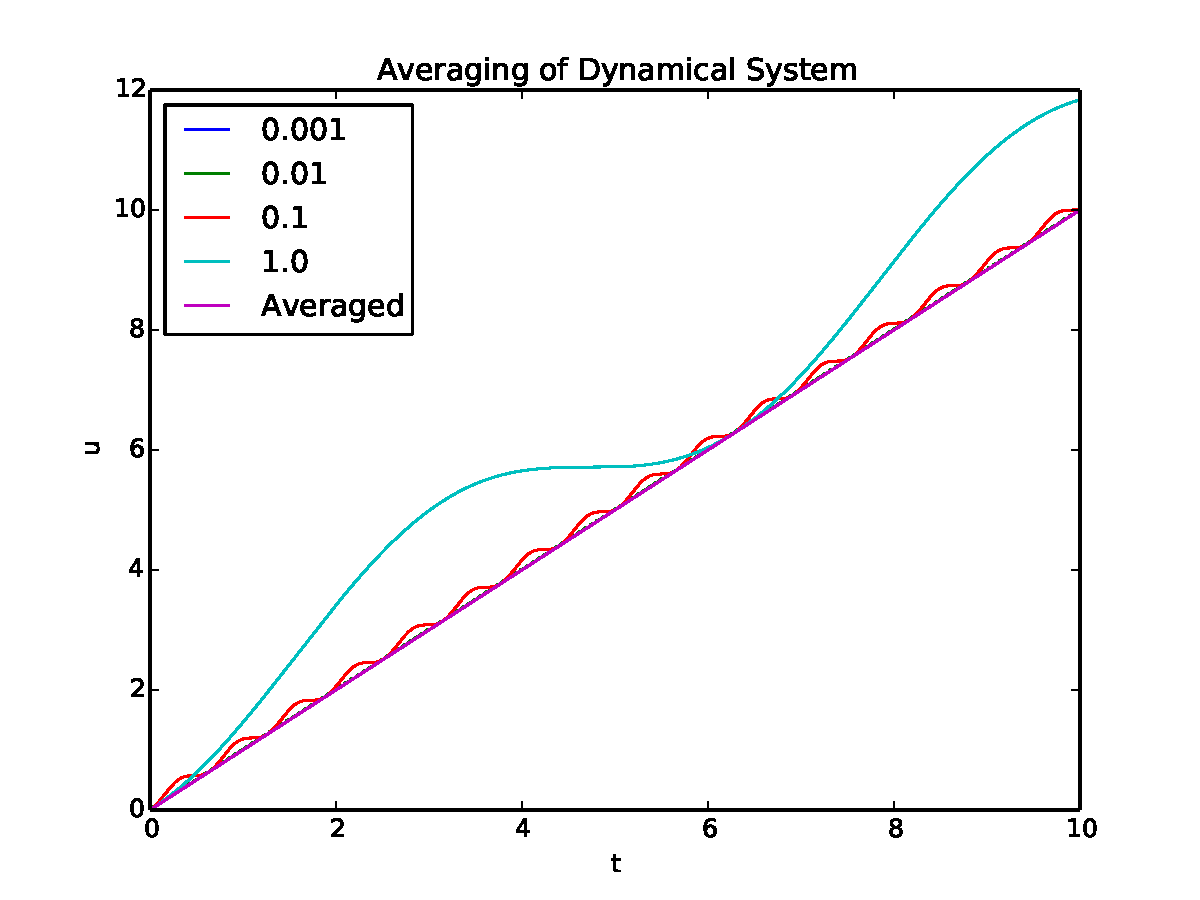
\includegraphics[width=\textwidth]{images/averaging.pdf}
    \caption{We see that as $\epsilon \to 0$, the oscillations lead to smaller and smaller discrepancy between the averaged and perturbed models}
    \label{fig:avgdynill}
\end{figure}

Qualitatively, this tells us that our solution is looks like the function $u_{\epsilon} = \bar{u} + p_{\epsilon}(t)$ where $p_{\epsilon}$ is an oscillatory term. As $\epsilon \to 0$, the oscillations matter less and less. This can be seen in Figure \ref{fig:avgdynill}. 

\subsection{Averaging of Coupled Dynamical System}
Here we consider a more complicated example. Consider the following coupled system of ODEs. 
\begin{align} \label{eqn:avgdyncoupled}
u_{t} &= v^2 & u(0) = 0 \label{eqn:top} \\
v_{t} &= \frac{1}{\epsilon} w & v(0) = 0 \label{eqn:middle} \\
w_{t} &= -\frac{1}{\epsilon} v & w(0) = 1 \label{eqn:bottom}
\end{align}
Note that we can decouple Equations \ref{eqn:middle} and \ref{eqn:bottom} and obtain harmonic oscillator models. The decoupling is achieved simply by differentiating both sides of each equation and substituting each of them into each other. Equation \ref{eqn:middle} becomes
\begin{ceqn} \label{eqn:middleuncoupled}
v_{tt} &= -\frac{1}{\epsilon^2} v \\
v(0) &= 0
\end{ceqn}
Equation \ref{eqn:bottom} becomes
\begin{ceqn} \label{eqn:bottomuncoupled}
w_{tt} &= -\frac{1}{\epsilon^2} w \\
u(0) &= 1
\end{ceqn}
We recover $v(t) = sin\left(\frac{t}{\epsilon}\right)$ and $w(t) = cos\left( \frac{t}{\epsilon} \right)$. Plugging these results and plugging into Equation \ref{eqn:top} and using trig identities, we obtain
\begin{align} \label{eqn:avgdyncoupledsoln}
u_{\epsilon}(t) = \frac{1}{2}\left(t - \frac{\epsilon}{2} sin\left(\frac{2t}{\epsilon}\right)\right).
\end{align}
We again take $\epsilon \to 0$ to get
\begin{align} \label{eqn:avgdyncoupledlimit}
\lim_{\epsilon \to 0} u_{\epsilon}(t) = \frac{t}{2} := \bar{u}(t).
\end{align}
Furthermore, we can derive a limiting differential equation as 
\begin{align} \label{eqn:avgdynlimiteqn}
u_{t} &= \frac{1}{2} \\
u(0) &= 0
\end{align}
This is a valid limiting equation that preserves all limits that we would like. However, the auxiliary variables $v$ and $w$ \textbf{do not have limiting equations!} Furthermore, if we were to average $v$ and $w$ before we were to plug them into Equation \ref{eqn:top}, then this would not work. It is thus important in this example that when we say ``limiting equation,'' we mean that we only take average as $\epsilon \to 0$ in Equation \ref{eqn:top}  with no other limits taken first. This example illustrates that we sometimes need to be careful in how we define limiting equations so that what we mean by ``asymptotic'' or ``averaging'' may need to be precisely defined to avoid misinterpretation of our limiting solution and/or limiting equation.

As a remark, we may note that $v^2 + w^2 = 1$ and is thus an invariant. As $\epsilon \to 0$, we simply observe that the solutions ``spin'' faster and faster around the unit circle.

We conclude this lecture by noting that the argument outlined here for this simple harmonic oscillator case can be generalized to the following equation.
\begin{ceqn} \label{eqn:avgdyncoupledgen}
u_{t}^{\epsilon} &= f(u^{\epsilon}, v^{\epsilon}) \\
v_{t}^{\epsilon} &= \frac{1}{\epsilon} g(u^{\epsilon}, v^{\epsilon}
\end{ceqn}
For fixed $u^{\epsilon}$, $v^{\epsilon}$ defines an invariant measure, albeit possibly more abstract than our previous case on the unit circle. From this we can recover that $u^{\epsilon} \to u$ where $u$ is the solution to
\begin{ceqn} \label{eqn:avgdyncoupledgenlimit}
u_{t} &= F(u) \\
F(u) := \int f(u,v) d\mu_{v}
\end{ceqn}
where $\mu_{v}$ is the invariant measure defined for fixed $u$. \askbjorn{Expand or leave here?}
\chapter{Lecture 9: Averaging of Dynamical Systems and Homogenization}
\section{Averaging of Dynamical Systems}
A more general system for averaging of dynamical systems from last lecture is the following system.
\begin{ceqn} \label{eqn:genavg}
u_{t}^{\epsilon} &= f(u^{\epsilon}, v^{\epsilon}) \\
v_{t}^{\epsilon} &= \frac{1}{\epsilon} g(u^{\epsilon}, v^{\epsilon}). 
\end{ceqn}
This gives a solution
\begin{align} \label{eqn:gensoln}
    u_{t} = F(u) = \int f(u,v) d\mu
\end{align}
where $\mu$ is an invariant \tcr{ in some sense...check with Bjorn.} As a remark, this form also generalizes to stochastic differential equations with adding $g \to g + c(u) dW$. Also, under the condition that $f$ is $T$-periodic,
\begin{align}
    u_{t} = \frac{\epsilon}{T} \int_{0}^{T} f(u,t,0) dt
\end{align}
\tcr{Is $\epsilon$ a characteristic scale? Why should the limiting solution depending on $\epsilon$? Bjorn will check on this.}
\subsection{Boosting}
$u^{\epsilon} \to u$ as $\epsilon \to 0$, but as $\epsilon \to 0$, we may induce extreme oscillatory behavior of the solution. These oscillations make recovery of the solution numerically difficult. Therefore, we have a tradeoff between these two factors so that we do not have to take extremely small time steps $\delta t \ll \epsilon$ in order to recover the solution. Some examples of this are the Car-Parinello method for molecular dynamics, added viscosity for the advection-diffusion equation, and the Kapitza pendulum. The Car-Parinello method artificially ``increases the mass of electrons'', which may be fine, but does not work for all molecules. As for the advection-diffusion equation, we can introduce an artificial viscosity  $\epsilon$ in the form
\begin{align} \label{eqn:advec}
    u_{t} + u_{x} = \epsilon u_{xx}.
\end{align}
For complex problems, this can be risky because the artificial viscosity term effectively changes the Reynolds number of the system of interest. This could mean you enter a turbulent regime when your true system should remain laminar. \tcr{It seems to me like there isn't an artificial viscosity term here...this just looks like a normal advection-diffusion equation with diffusivity constant $\epsilon$.} The Kapitza pendulum is an inverted pendulum which has an unstable equilibrium point at $\theta = 0$. If we drive the pendulum vertically, then we can stabilize this equilibrium point. This leads to a system of the form
\begin{align}
    \ddot{\theta} = \left(D\omega^2cos(\omega t) - \frac{D}{l}\right) sin(\theta).
\end{align}
Here, there is a critical value for $\omega$ that will stabilize the equilibrium position, similar to how Reynolds number creates a critical regime for turbulence.
\section{Homogenization}
Homogenization can be thought of as an ``oscillation in space'' for many applications. \tcr{Check with Bjorn on this statement, if we want to expand...his example shows the oscillation in space, but does it ALWAYS require periodicity for homogenization to be applicable?}

As an example, consider an elliptic problem of the form
\begin{ceqn} \label{eqn:9:ellipeps}
& - \nabla \cdot (a(\bs{x},\frac{\bs{x}}{\epsilon}) \nabla u^{\epsilon}) = f(\bs{x}) \\
& + (\tu{whatever boundary condition we want here})
\end{ceqn}
where $a(x,y)$ is $1$-periodic in $y$, i.e. $a(x,y+1) = a(x,y)$ for all $y$.
Applications for this type of problem are in composite materials and flow in porous media. Homogenization seeks to map $a(x,\frac{x}{\epsilon}) \to A(x)$ such that solutions $u^{\epsilon} \to u$ where $u$ is given by 
\begin{ceqn} \label{eqn:elliplimit}
& -\nabla \cdot (A(\bs{x}) \nabla u(\bs{x})) = f(\bs{x}) \\
& + \tu{appropriate BC  based on \eqref{eqn:ellipeps}}
\end{ceqn}
We now work out the details of a one-dimensional example with $a(x,y) = a(y)$ and homogeneous Dirichlet boundary conditions. That is,
\begin{ceqn} \label{eqn:homoeps}
& -\frac{d}{dx}\left( a\left(\frac{x}{\epsilon}\right) \frac{du^{\epsilon}}{dx}\right) = f(x) & x \in (0,1) \\
& u(0) = u(1) = 0 & 
\end{ceqn}
\begin{figure}
    \centering
    
\includegraphics{images/x.pdf}
    \caption{Insert oscillatory graphic of $a(\frac{x}{\epsilon})$}
    \label{fig:homooscil}
\end{figure}
We seek a homogenized equation of the form
\begin{ceqn}
& -\frac{d}{dx}\left( \tilde{a} \frac{du}{dx} \right) = f & x \in (0,1) \\
& u(0)=u(1)=0 &
\end{ceqn}
where $\tilde{a}$ is an appropriate chosen constant. A natural choice would be to choose $\tilde{a}$ to be the simple average given by
\begin{align} \label{eqn:constawrong}
\tilde{a} = \frac{1}{\epsilon}  \int_{0}^{\epsilon} a\left(\frac{x}{\epsilon}\right) dx = \int_{0}^{1} a(\xi) d\xi.
\end{align}
However, as we will see, this is an incorrect choice for $\tilde{a}$. Integrate \eqref{eqn:homoeps} once to obtain
\begin{align} \label{eqn:homoepsint1}
-a\left(\frac{x}{\epsilon}\right) \frac{du^{\epsilon}}{dx} = \underbrace{C + \int_{0}^{x} f(\xi) d\xi}_{F(x)}.
\end{align}
Now simply divide by $a$ and then integrate again to obtain
\begin{align} \label{eqn:homoepsint2}
    u^{\epsilon}(x) = -\int_{0}^{x} \frac{F(\xi)}{a\left(\frac{\xi}{\epsilon}\right)} d\xi
\end{align}
where we have applied the boundary condition $u(0) = 0$ to get rid of the integration constant. Let $N = \lfloor \frac{x}{\epsilon} \rfloor$. Rewrite \eqref{eqn:homoepsint2} as 
\begin{align} \label{eqn:homoriem}
    u^{\epsilon}(x) &= -\underbrace{\int_{N\epsilon}^{x} \frac{F(\xi)}{a\left(\frac{x}{\epsilon}\right)} d\xi}_{g(x,\epsilon)} - \sum_{n=0}^{N-1} \int_{n\epsilon}^{(n+1)\epsilon} \frac{F(\xi)}{a\left(\frac{x}{\epsilon}\right)} d\xi & \nonumber \\
    &= g(x,\epsilon) - \underbrace{\epsilon \sum_{n=0}^{N-1}\int_{n\epsilon}^{(n+1)\epsilon} \frac{F'(s(\xi))}{a\left(\frac{\xi}{\epsilon}\right)}}_{h(\epsilon)} - \sum_{n=0}^{N-1} F(n\epsilon) \int_{n\epsilon}^{(n+1)\epsilon} \frac{1}{a\left(\frac{x}{\epsilon}\right)} 
\end{align}
where $s(\xi)$ is given by the mean-value theorem. Continuing with simple substitution, we have
\begin{align} \label{eqn:homoriem2}
u^{\epsilon}(x) &= g(x,\epsilon) - h(\epsilon) + \epsilon \sum_{n=0}^{N-1} F(n\epsilon) \int_{n}^{n+1} \frac{1}{a(\xi)} d\xi \nonumber &\\
&= g(x,\epsilon) - h(\epsilon) - \underbrace{\left( \int_{0}^{1} \frac{1}{a(\xi)}d\xi\right)}_{\tilde{a}} \sum_{n=0}^{N-1} F(n\epsilon) \epsilon & (a \tu{ is } 1\tu{-periodic}).
\end{align}
Now take $\epsilon \to 0$ in \eqref{eqn:homoriem2}. If we assume that $f$ is continuous and $a$ is bounded below, then both $g(x,\epsilon) \to 0$ and $h(\epsilon) \to 0$, which we leave as an exercise for the reader. We  simply note that we only have a Riemann sum left, and thus $u^{\epsilon}$ indeed converges to a limiting function $u$ given by
\begin{align} \label{eqn:homolimit}
    u(x) = -\tilde{a} \int_{0}^{x} F(\xi) d\xi.
\end{align}
Note further that $u^{\epsilon}(1) = u^{\epsilon}(0) = 0$, so $u(1) = u(0) = 0$ also.
Differentiating \eqref{eqn:homolimit} twice, we recover the BVP
\begin{ceqn} \label{eqn:odelimit}
& -\frac{d}{dx} \left( \tilde{A} \frac{du}{dx} \right) = f(x) \\
& u(0) = u(1) = 0.
\end{ceqn}
where $\tilde{A} = \frac{1}{\tilde{a}}$ is the \tbf{harmonic average} of $a$, rather than the immediate approach of the standard average.
\chapter{Lecture 10}
\section{\tcr{A bit confused on this part, related to homogenization}}

\section{Outline of Future Lectures}
Next lecture will be our last class that covers mapping models to other models. We will move onto the following topics:
\begin{itemize}
    \item Model reduction
    \item Reduced-order modeling
    \item Metamodels
    \item Surrogate models.
\end{itemize}
These topics are similar to each other and a large extent, are really the same thing under a different name \askbjorn{double check that my understanding is correct, items 1,2, and 4 seem essentially the same, but I'm unsure about item 3}. The goal of these approaches is to map a complex model to a simpler one. For example, rather than capturing the full solution to a PDE, we can approximate it best the best rank $r$ approximation for small $r$ via a singular-value decomposition. Some important aspects to keep in mind when performing such a reduction are listed below.
\begin{itemize}
    \item Reduced accuracy of the solution
    \item Reduced-order model should preserve important solution properties, e.g., conservation of mass
    \item Reduced-order model should preserve well-posedness
\end{itemize}
Some common techniques include
\begin{itemize}
    \item Projection onto a lower-dimensional subspace, e.g., truncated SVD
    \item \tcr{Exploit par. dep. --> ``parametric dependence''?}
    \item Divide solution into online and offline calculation\footnote{\tcr{Expand explanation here in footnote. Basically, you want your online stage to be a simpler model, e.g., a homogenized form of the equation}}.
    \item Exploit small parameters after transformation, e.g., setting small singular values to $0$, dropping a term from differential equation as negligible, etc.
\end{itemize}
\chapter{Lecture 11}
Continuing from the end of last lecture, we go into more detail on reduced-order modeling.

\section{Example: Fast Models in Control Theory}
We consider the following ODE that is typical of control theory.
\begin{ceqn} \label{eqn:11:controlODE}
\dot{x}(t) &= f(x(t), u(t)) \\
y(t) = g(x(t), u(t)).
\end{ceqn}
In our context, $u,y$ are low dimensional and $x$ is high dimensional. For example, $x$ could be the temperature field of an entire building, $u$ the internals of a thermostat device, and $y$ a switch to change the thermostat state. Fast models in control theory exploit this dimensionality difference to create fast solvers for $y$. Note that $y$ is the value of most direct interest since it is the only thing we have direct control over in the context of control theory. $y$ will usually represent something such as a light switch, a joystick for something such as a crane, a thermostat control, etc.

\section{Example: Linear System}
Reduced-order modeling is often applied to solving PDEs whose solution ultimately reduces to solving a linear system. Therefore, let's look simply at a linear system with a setup typical of one that might be seen in the context of a PDE. 
\begin{ceqn} \label{eqn:11:linear}
\bs{L} \bs{x} &= \bs{f} \\
\begin{bmatrix}
\bs{A} & \bs{B} \\
\bs{C} & \bs{D}
\end{bmatrix}\begin{bmatrix}
\bs{x}_{1} \\
\bs{x}_{2}
\end{bmatrix} &= \begin{bmatrix}
    \bs{f}_{1} \\
    \bs{f}_{2}
\end{bmatrix} \\
\bs{x}_1 \in \R^{m_1},& \textup{ } \bs{x}_2 \in \R^{m_2}  \\
\bs{f}_1 \in \R^{n_1},& \textup{ } \bs{f}_2 \in \R^{n_2}.
\end{ceqn}
In our context, we assume $m_1 \gg m_2$. This leads to the following two equations.
\begin{align} 
\bs{A} \bs{x}_1 + \bs{B} \bs{x}_2 &= \bs{f}_1 
    \label{eqn:11:blockbreak1} \\
\bs{C} \bs{x}_{1} + \bs{D} \bs{x}_2 &= \bs{f}_2.
    \label{eqn:11:blockbreak2}
\end{align}
The solution to Equation \ref{eqn:11:blockbreak1} is
\begin{align} \label{eqn:11:blockbreak1soln}
\bs{x}_1 &= \bs{A}^{-1} \left( \bs{f}_{1} - B \bs{x}_2 \right).
\end{align}
Plugging Equation \ref{eqn:11:blockbreak1soln} into Equation \ref{eqn:11:blockbreak2} gives
\begin{align} \label{eqn:11:blockbreak2soln}
\left( \bs{D} - \bs{C} \bs{A}^{-1} \bs{B} \right) \bs{x}_{2} &= \bs{f}_2 - \bs{C} \bs{A}^{-1} \bs{f}_1.
\end{align}
Note that $\bs{A}$ is a large matrix, so we want to compute with it as little as possible. Therefore, we compute $\bs{D} - \bs{C} \bs{A}^{-1} \bs{B}$ and $\bs{C} \bs{A}^{-1}$ offline and then solve Equation \ref{eqn:11:blockbreak2soln} online. This will have significant savings in the case when we have many right hand sides of the form Equation \ref{eqn:11:blockbreak2soln}, otherwise it will likely not be worth performing this strategy. Note further that in the case that $A$ is too large to store, we can still perform this online/offline approach if we only know the action of $A$. For each column of $\bs{b}_i$ of $B$, we can solve the equation
\begin{align} \label{eqn:11:toolarge}
\bs{A} \bs{u}_{i} = \bs{b}_i
\end{align}
via an appropriate iterative solver, e.g., a Krylov subspace method such as GMRES.
\chapter{Lecture 12}
In this lecture, we continue with our discussion of reduced-order models which are a method of mapping models to models. In this lecture, we look at problems where we seek a reduced basis that represents the solution to our problem as well as projections into that basis. Examples of such projections include the singular-value decomposition, eigenbases, Krylov-subspace methods, and the Hankel transform.

\section{Example: Wavelet Transform}
Consider the linear system of equations
\begin{align} \label{eqn:12:linear}
\bs{L} \bs{u} = \bs{f}
\end{align}
Let $W$ be the matrix representing a wavelet transform. Since $W$ is unitary, we can rewrite
\begin{align} \label{eqn:12:waveletlinear}
\bs{W}\bs{L}\bs{W}^{*} \tilde{\bs{u}} &= \bs{\tilde{f}}
\end{align}
with $\tilde{\bs{u}} = \bs{W} \bs{u}$ and $\bs{\tilde{f}} = \bs{W}\bs{f}$. Since $\bs{\tilde{f}}$ is now in the wavelet basis, we can reshuffle its components so that its high-frequency components appear first. That is, we can use a unitary $\bs{Q}$ so that
\begin{align} \label{eqn:12:unitary}
\bs{Q} \bs{W} \bs{L} \bs{W}^{*} \bs{Q} \bs{\bar{u}} &= \bs{\bar{f}}
\end{align}
where $\bs{\bar{f}} = \bs{Q} \bs{\tilde{f}} = \bs{Q} \bs{W} \bs{f}$ and $\bs{\bar{u}} = \bs{Q} \bs{\tilde{u}} = \bs{Q} \bs{W} \bs{u}$. Finally, rewrite Equation \ref{eqn:12:unitary} as
\begin{align}
\begin{bmatrix}
\bs{A} & \bs{B} \\
\bs{C} & \bs{D}
\end{bmatrix} \begin{bmatrix}
    \bs{u}_{H} \\
    \bs{u}_{L}
\end{bmatrix} &= \begin{bmatrix}
\bs{f}_{H} \\
\bs{f}_{L}
\end{bmatrix} \\
\bs{u}_{H}, \bs{f}_{H} \in \R^{n_1} \\
\bs{u}_{L}, \bs{f}_{L} \in \R^{n_2}
\end{align}
with $n_1 \gg n_2$ and 
\begin{align}
    \begin{bmatrix}
    \bs{A} & \bs{B} \\
    \bs{C} & \bs{D}
    \end{bmatrix} = \bs{Q} \bs{W} \bs{L} \bs{W}^{*} \bs{Q}^{*}.
\end{align}
Here, we use the subscript $H$ to mean ``high frequency'' and $L$ to mean ``low frequency.'' Typically, noise lies in the high-frequency range, and so we are only interested in solving for $u_L$ and throwing away $u_H$, even though $dim(u_H) \gg dim(u_L)$!
From here, we can apply the same online/offline strategy outlined in the previous lecture. Again this approach is of practical use for many right hand sides $\bs{u}_L$.

\section{Example: Control Theory}
Consider Equation \ref{eqn:11:controlODE} from Lecture 11. We begin in the case when $f,g$ are linear. Then Equation \ref{eqn:11:controlODE} becomes
\begin{ceqn} \label{eqn:12:linearcontrol}
\dot{\bs{x}}(t) &= \bs{A} \bs{x}(t) + \bs{B} \bs{u}(t) \\
y(t) &= \bs{C} \bs{x}(t) + \bs{D} \bs{u}(t)
\end{ceqn}
with $dim(\bs{x}) \gg dim(\bs{y})$. Consider the case when $\bs{B} = \bs{D} = \bs{0}$ so that we have the further reduction
\begin{align} 
\dot{\bs{x}}(t) &= \bs{A} \bs{x}(t) \label{eqn:12:nou1} \\
\bs{y}(t) &= \bs{C} \bs{x}(t) \label{eqn:12:nou2}
\end{align}
We note that Equation \ref{eqn:12:nou2} leads to a drastic dimensionality reduction through the matrix $\bs{C}$. Is there any way that we can incorporate $\bs{C}$ into Equation \ref{eqn:12:nou1} to lead to an overall complexity reduction? We can see through straightforward algebra that
\begin{align} \label{eqn:12:reducey}
\dot{\bs{y}}(t) &= \bs{C} \bs{A} \bs{x}(t).
\end{align}
Note that the right-hand side of Equation \ref{eqn:12:reducey} does not have $\bs{y}$, so we do not see a direct dimensionality reduction from this equation, and for general $\bs{A}$, we cannot expect any reduction.   
\chapter{Lecture 13}
We begin with a few remarks regarding ROM. We typically have a sparse structure in our original problem that we are reducing\footnote{Because we are typically looking at a matrix equation arising from the discretization of a PDE. Since differentiation is a local operator, we typically see sparse matrices.}. However, this sparse structure is lose when we take the SVD or EVD. This loss of sparsity means that we can only justify attempting a reduced-order model if either (a) the order of the problem is drastically reduced or (b) the order is moderately reduced but is applied to many right hand sides to where the loss of sparsity is worth the tradeoff. However, in special cases, the sparsity can be preserved, which is ideal.

\section{Example: Preservation of sparsity in multiscale FEM}
Consider the following model equation.
\begin{align} \label{eqn:13:model}
-\frac{d}{dx} \left( a(\frac{x}{\epsilon}) \frac{du_{\epsilon}}{dx} \right) = f.
\end{align}
We assume $a$ is oscillatory. Multiscale FEM uses a reduced basis $\mathcal{C} := \{\psi_{k}\}$ ($\mathcal{C}$ here denotes ``coarse'') with $h_{\psi} \gg h_{\phi}$ where $\mathcal{F} := \{\phi_{j}\}$ ($\mathcal{F}$ here denotes ``fine'')is a reference basis and the support of each basis function is $O(h_{\psi}),O(h_{\phi})$ for $\{\psi_{k}\}, \{\phi_{j}\}$, respectively. Also, $\psi_{k}$ is typically a linear combination of the elements of $\mathcal{F}$ for each $k$. The coarse basis $\mathcal{C}$ is used to cheaper solve for coarse-scale structure and $\mathcal{F}$ for fine-scale structure, illustrated in Figure \ref{fig:13:multiscalefem}. Since each basis still has local support, the sparsity is preserved for the coarse-scale operation. This approach has gain only when considering many right hand sides $\bs{f}$ since we only have to solve the matrix equation recovering $\mathcal{C}$ from $\mathcal{F}$ once, independent of the number of right hand sides we have. \askbjorn{Is the gain from the fact that we use the same approach in the matrix solve as outlined in previous lectures?} 
\begin{figure}
    \centering
    
\includegraphics{images/x.pdf}
    \caption{Want a simple hat function with a bunch of oscillations in it. The coarse basis will be the hat function and the fine basis is able to capture the intermediate oscillations.}
    \label{fig:13:multiscalefem}
\end{figure}
Extensions to this idea exist in higher dimensions. However, the geometry of extracting a coarser basis gets markedly more complicated even in two dimensions, so we omit for the sake of this course. \askbjorn{Any references for students who may be interested in this?}

\section{Example: Maxwell's Equation}
Another example where sparsity can be preserved is with boundary integral equation (BIE). In short, boundary integral equations solve an $(n+1)$-dimensional problem by using Green's theorem to reduce to an $n$-dimensional problem on the boundary of the domain of interest. A finite-difference discretization of the problem will lead to a sparse matrix inversion problem. When pulled onto the boundary via Green's Theorem, we get a dense problem but with less degrees of freedom. For any point $x$ in the domain, we can calculate via an appropriate Green's function that
\begin{align} \label{eqn:13:BIE}
    \rho(x) = \int_{\Gamma} K(x,y) \rho(y) dy
\end{align}
where $\Gamma = \partial \Omega$ is the boundary of domain $\Omega$. However, we can then approximate this kernel evaluation with the fast multipole method which leads to a sparse compression. Overall, then we can reduce a three-dimensional sparse matrix inversion problem to a sparse two-dimensional sparse \textbf{matvec}! This is a huge reduction in complexity. We note that knowledge of the Green's function is necessary to apply a BIE formulation, restricting the class of problems for which it can be applied. However, we note that it is reasonable approximation for air to be a homogeneous medium, which means that this method can be applied to wireless communication, given that the Green's function for a homogeneous medium is known.
\chapter{Lecture 14}
We cover wellposedness in this lecture. As a review, we consider a problem well-posed whenever (a) solutions exist, (b) solutions are unique, and (c) solutions depend continuously on initial conditions.

\section{Wellposedness of ODEs}
Consider the simple ODE below.
\begin{ceqn} \label{eqn:14:ODE}
y'(t) &= f(y(t)) & t \in (0,T) \\
y(0) &= y_0.
\end{ceqn}
The wellposedness of this problem depends on the forcing function $f$. For example, whenever $f(y) = 2\sqrt{y}$, solutions exist but are not unique. If we take $y_0 = 0$, we see that $y(t) \equiv 0$ and $y(t) = t^2$ both solve Equation \eqref{eqn:14:ODE}. In general, $f$ Lipschitz is a sufficient condition for wellposedness and can be shown Picard iteration. Here, we outline the proof of showing continuous dependence on data. To prove this, we need Gronwall's inequality, stated below.
\begin{lemma}{(Gronwall's Inequality)} \label{thm:14:gronwall}
Let $u$ and $\beta$ be continuous on an interval $I$ which contains its infimum. Suppose $u$ is differentiable on $I^{0}$, the interior of $I$, and satisfies the differential inequality 
\begin{align} \label{eqn:gronwall}
u'(t) \leq \beta(t) u(t)
\end{align}
on $I^{0}$. Then for all $t \in I$,
\begin{align}
    u(t) \leq u(a) \int_{a}^{t} \beta(s) ds
\end{align}
\end{lemma}
\begin{theorem}
If $f$ is Lipschitz continuous, then solutions to Equation \eqref{eqn:14:ODE} depend continuously on the initial condition.
\end{theorem}
\begin{proof}
Let $y$ solve Equation \eqref{eqn:14:ODE} with initial condition $y(0) = y_0$ and let $u$ solve Equation \eqref{eqn:14:ODE} with initial condition $u(0) = y_0 - \epsilon$. Then for any $t \in (0,T)$, we have
\begin{ceqn} \label{eqn:14:derivbound}
    y'(t) - u'(t) &= f(y(t)) - f(u(t)) \\
    &\leq |f(y(t)) - f(u(t))| \\
    &\leq L |y(t) - u(t)|
\end{ceqn}
Note that $y(0) - u(0) = \epsilon$. Denoting $E(t) = y(t) - u(t)$, we can thus rewrite Equation \eqref{eqn:14:derivbound} as 
\begin{ceqn} \label{eqn:14:errinequal}
     E'(t) &\leq L |E(t)| \\
     E(0) &= \epsilon
\end{ceqn}
Applying Lemma \ref{thm:14:gronwall}, we have for any $t \in [0,T]$
\begin{ceqn}
E(t) &\leq \epsilon e^{L(t-a)} \\
&\leq M \epsilon
\end{ceqn}
where $M = e^{LT}$. Therefore, we have continuous dependence in $L^{\infty}$ and thus also all $L^{p}$ norms.
\end{proof}
\chapter{Lecture 15}
\section{Continuous Depedence on Data}

\section{Sensitivity Analysis}
Sensitivity analysis gives more information than simply continuous dependence on data. Generally speaking, sensitivity analysis relates specific components of input to their associated outputs. \tcr{This is easiest to see in terms of the SVD (write up later)}. Consider
\begin{ceqn} \label{eqn:15:sensitive}
    f(\bs{x} + \Delta \bs{x}) &= \bs{y} + \Delta \bs{y} \\
    &\approx f(\bs{x}) + \nabla f(\bs{x}) \cdot \Delta \bs{x} + (\Delta \bs{x})^{T} \bs{H}(\bs{x}) \Delta \bs{x}.
\end{ceqn}
Matching first-order terms, we have
\begin{align} \label{eqn:15:firstorderperturb}
\Delta \bs{y} \approx \nabla f(\bs{x}) \cdot \Delta \bs{x}
\end{align}

\section{Uncertainty Quantification (UQ)}
The overarching goal of uncertainty quantification (UQ) is to obtain \textbf{statistical information of solution from statistical information of data}, e.g. expected value, variance, probability density, etc. UQ is typically expressed in the language of probability and statistics. For random variable $X$, we define its cumulative distribution function (CDF) as 
\begin{align} \label{eqn:15:cdf}
    F_{X}(x) = \mathbb{P}(X \leq x).
\end{align}
Whenever the CDF is differentiable, we denote its derivative as $f_{X}(x)$ and call it its probability density function (PDF). The CDF can also be recovered from the PDF as
\begin{align}
F_{X}(x) = \int_{-\infty}^{x} f_{X}(t) dt.
\end{align}

\subsection{Remark on power of UQ}
The conditioning of our model can tell us some information for two extremes. That is if we know that our input is distributed by a random variable $X$, then all the condition number can tell us is that our output distribution lies somewhere in $[-K \delta, K \delta]$ where $K$ is our condition number and $\delta$ is the length of the support of $X$, assuming, for simplicity, that the support is compact. UQ seeks to create a complete picture of this mapping from input distribution $X$ to another random variable $Y$ describing the output distribution.

\section{UQ Techniques}
\begin{itemize}
    \item Analytic Derivation
    \item Monte Carlo (sampling)
    \item Reduced-order modeling
    \item Reduced basis (expansions, e.g., Karhonnen-Lo\`{e}ve)
    \item Interval analysis (this is a bit more exotic)
\end{itemize}

\subsection{Support Estimation}
Consider the problem of estimating the support of the output density given the support of the input probability density. \tcr{Fill in these details later...main idea is that if you know the range of the inputs, you can deterministically determine when we get nonzero output...note that this is also in a probability 1 sense}. 

\subsection{Analytic Derivations}
In some circumstances, we can analytically derive the output distribution from the input distribution.
Suppose that our output is given by 
\begin{align} \label{eqn:15:uniform}
Z = X + Y
\end{align}
where $X \sim U(0,1)$ and $Y \sim U(0,1)$ are independent inputs. Then we can immediately calculate the PDF of $Z$ as \begin{ceqn} \label{eqn:15:density}
    f_{Z}(z) &= \int_{-\infty}^{\infty} f_{X}(\xi) f_{Y}(z-\xi) d\xi \\
    &= z \mathds{I}_{[0,1]}(z) + (2-z) \mathds{I}_{(1,2]}(z)
\end{ceqn}
where $I$ is the indicator function.


\chapter{Lecture 16}
\chapter{Lecture 17}
We continue our discussion of UQ from last lecture.
\section{Analytic Methods Continued}
Consider the stochastic differential equation
\begin{ceqn} \label{eqn:17:sde}
    y'(t) &= f(y(t)) + r(t) \\
    y(0) &= y_0.
\end{ceqn}
For simplicity, set $f \equiv 0$. Since $r(t)$ is not continuous, Equation \eqref{eqn:17:sde} does not make sense. We must, therefore, cast to a properly defined stochastic differential equation with \^{I}to calculus as
\begin{align} \label{eqn:17:ito}
    dF_{t} = \sigma(F_t) dW_t \overset{const.}{=} \sigma dW_t.
\end{align}
This stochastic differential equation can be recast to the Fokker-Planck Equation, stated below.
\cbeqn{Fokker-Planck Equation}{
    \frac{\partial}{\partial t}\left( r_{F}(x,t) \right) = \frac{\partial^2}{\partial x^2} \left( \sigma^2 r_{F}(x,t) \right) \label{eqn:17:fokker}
} 
Here, $r_{F}$ is a probability density function that describes the stochastic process $F$. \askbjorn{should I comment on why we have two variables here? I don't recall why we have two variables.} Equation \eqref{eqn:17:ito} solves for a specific trajectory of the stochastic process $F_t$. Therefore, to get a picture of this process, we must perform a Monte Carlo simulation. However, the Fokker-Planck equation \textit{directly} solves for the PDF that describes $F$! This is another example of a mapping from a model to another model. 

\section{Monte Carlo Continued}
\subsection{Importance Sampling}
Consider $Z = X + Y$ where $X \sim U(0,1)$ and $Y \sim U(2,3)$ with $X$ and $Y$ independent. If we want to approximate $Z$, sampling from intervals outside of $[0,1] \cup [2,3]$ gives us less information than sampling from $[0,1]\cup[2,3]$...\askbjorn{This would be illustrative example, but you have to make sure you think about the sample space properly.}

Now let us consider the slightly more complicated example of Monte Carlo integration. That is, we want to compute the value $\mathbb{E}\left[ f(X) \right]$ as 
\begin{align} \label{eqn:17:MCint}
    \int_{\Omega} f(x) dx \approx S_{N} := \frac{|\Omega|}{N} \sum_{n=1}^{N} f(x_n)
\end{align}
where $\Omega$ is our sample space and $x_n$ are selected uniformly from $\Omega$ and in i.i.d. fashion, i.e. $X \sim U(\Omega)$ (\askbjorn{cross reference this}). The sample standard deivation estimates the error of this calculation. That is,
\begin{align} \label{eqn:err_importance}
    \left|\EE{f(X)} - S_{N}\right| \sim \sqrt{\frac{Var(f)}{N}}.
\end{align}
Importance sampling is based off simply considering a different form of Equation \eqref{eqn:err_importance} as
\begin{align} \label{eqn:err_controlvar}
\left|\EE{\frac{f(X)}{g(X)}} - S_{N} \right| \sim \sqrt{\frac{1}{N} Var\left[\frac{f(X)}{g(X)}\right]}.
\end{align}
Note that whenever $g \approx f$, we have that 
\begin{align*}
    Var\left[\frac{f(X)}{g(X)}\right] < Var(f(X)).
\end{align*}
If $g$ is chosen appropriately, we may reduce the variance for a given computational cost budget. \askbjorn{Insert figure that you did for Richard Tsai's class that illustrates this}. We can rewrite
\begin{ceqn} \label{eqn:17:stieltjes}
\int_{\Omega} f(x) dx &= \int_{\Omega} \frac{f(x)}{g(x)} g(x) dx \\
&= \int_{\Omega} \frac{f(x)}{g(x)} \underbrace{d\mu_{g}(x)}_{\textup{Stieltjes}} \\
&\approx \frac{|\Omega|}{N} \sum_{n=1}^{N} \frac{f(x_n)}{g(x_n)}.
\end{ceqn}
In Equation \eqref{eqn:17:stieltjes}, the $x_n$ are now i.i.d. samples taken from the measure $\mu_g$. This alternative sampling from $\mu_g$ picks out the more \q{important} regions that characterize the distribution than a uniform sampling and thus motivates the phrase \q{importance sampling.} Another related term to Google is \textbf{control variates} \askbjorn{Is this correct? Is there a difference between control variates and importance sampling?}

Note that in the case that $g=f$, we get zero variance and we immediately recover the correct answer. However, in Equation \eqref{eqn:17:stieltjes}, we must sample from $\mu_{g}=\mu_{f}$ $N$ times. However, this presupposes that the value of the integral is known a priori and is thus useless. \askbjorn{There seems an inconsistency here...I am misunderstanding something now or misunderstood something said during lecture}. 

An example where importance sampling is used is with exit polls. \askbjorn{Create figure for this.}

Another example is uncertainty quantification for rare events. For hurricanes, you would ideally take $g$ to be under warmer conditions to bias towards hurricane formation.

\section{Multilevel Monte Carlo}
Mulitilevel Monte Carlo (MLMC) is a variance reduction technique that allows for possibly greater gains than the previous section regarding importance sampling.
Say we want to estimate the mean of a given random variable $X$ from which sampling is an expensive operation.
This can be achieved directly by simply taking $N$ samples as we discussed in the previous section. That is,
\begin{align} \label{eqn:17:directmlmc}
\EE{X} \approx S_N \approx \frac{1}{N} \sum_{n=1}^{N} X(x_n)
\end{align}
where $x_n \in \Omega$ is chosen uniformly from the sample space $\Omega$. 
Note that
\begin{align*}
    Var(S_N) = \frac{Var(X)}{N}
\end{align*}
and so we have that
\begin{align} \label{eqn:17:rms}
\EE{(X-S_N)^2} &= Var(S_N) = \frac{Var(X)}{N} = O\left(\frac{1}{N}\right).
\end{align}
This leads to a fundamental Monte Carlo result that
\cbeqn{Na\"{i}ve Monte Carlo RMS Error}{
    E_{rms} := \sqrt{\EE{(X-S_N)^2}} = \sqrt{\frac{Var(X)}{N}} = O(N^{-1/2}) \label{eqn:17:mcrms}
} 
If we would like to think of how many samples we must use to get a specified error, we have a simple corollary stated below.
\cbeqn{Na\"{i}ve MC RMS cost estimate}{
    \textup{For } E_{rms} \leq \epsilon, \textup{ we must take } N=O(\epsilon^{-2}) \textup{ samples.}
}
Our goal with MLMC is to improve upon the cost associated with Equation \eqref{eqn:17:mcrms}. 
Define a sequence of approximations to $X$ as $X_0,...,X_L$ where $X_{l-1} \approx X_{l}$ and $X_L=X$.
Then we can simply write the telescopic sum 
\begin{align} \label{eqn:17:telescope}
    \EE{X} = \EE{X_{N}} = \EE{X_0} + \sum_{l=1}^{L} \EE{X_{l} - X_{l-1}}.
\end{align}
From here, we can derive the unbiased estimator
\begin{align} \label{eqn:17:estimate}
    \hat{X} = \hat{X}(N_0,N_1,...,N_L) = \frac{1}{N_0} \sum_{n=1}^{N_0} X_{0}^{(0,n)} + \sum_{l=1}^{L}\left[ \frac{1}{N_l} \sum_{l=1}^{N_l} \left(X_{l}^{(l,n)} - X_{l-1}^{(l,n)}\right) \right].
\end{align}
Our question of interest now is \q{for a fixed RMS error $\epsilon$, what choice of $N_0,...,N_L$ will lead to the least computational cost?} The optimal choice is given by
\begin{ceqn} \label{eqn:17:mlmcchoice}
    N_{l} &= \mu \sqrt{\frac{V_l}{C_l}} \\
    \mu &= \frac{1}{\epsilon^2} \sum_{l=0}^{L} \sqrt{V_l C_l}.
\end{ceqn}
Equation \eqref{eqn:17:mlmcchoice} leads to a total cost of 
\cbeqn{MLMC computational cost estimate}{
    \textup{For } E_{rms} \leq \epsilon, \textup{ cost } C=\epsilon^{-2} \left( \sum_{l=0}^{L} \sqrt{V_l C_l} \right)^2 \label{eqn:17:mlmccost}
}
Equation \eqref{eqn:17:mlmcchoice} implies the following savings expressed as a ratio of the MLMC cost, $C_{MLMC}$, and the traditional, direct Monte Carlo estimation cost, $C_{MC}$.
\cbeqn{MLMC Savings - First Level Dominant}{
    V_0 C_0 \textup{ dominant in Equation } \eqref{eqn:17:mlmccost} \Rightarrow \frac{C_{MLMC}}{C_{MC}} \approx \frac{V_L}{V_0} \label{eqn:17:mlmcsavfirst} 
}
\cbeqn{MLMC Savings - Last Level Dominant}{
    V_L C_L \textup{ dominant in Equation } \eqref{eqn:17:mlmccost} \Rightarrow \frac{C_{MLMC}}{C_{MC}} = \frac{C_0}{C_L} 
}
Equations \eqref{eqn:17:mlmcsavfirst} and \eqref{eqn:17:mlmccost} will express savings whenever our equation is less than unity. By design, we choose $C_0 < C_1 < C_2 < ... < C_L$ and $V_0 > V_1 > V_2 > ... > V_L$. This relationship is inverted because to observe less variance, we typically need more samples. However, we note that if these constraints are not met in practice, then we will not expect MLMC to give us any computational savings. More details on this topic can be found in the paper \textit3{Multilevel Monte Carlo Methods} by Michael Giles. 

\chapter{Lecture 18}
In this lecture, we discuss model complexity. Model complexity can fall into many categories including, but not limited to, the following items.
\begin{itemize}
    \item Analysis 
    \item Can the model be approximated well with a simpler model?
    \item How costly is the model to compute?
    \begin{itemize}
        \item Computational complexity for problem class (e.g., P or NP?)
        \item Computer time cost 
        \item Basic operation count (number of floating point operations)
        \item Memory requirements (e.g., solving linear system iteratively requires less memory than LU factorization)
        \item Parallelizability
    \end{itemize}
\end{itemize}
Note that regarding computing cost, we often consider worst-case, best-case, and average-case scenarios. For example, for optimizing a function $f$, simplex methods have a very large worst-case cost but have reasonable average-case cost.
\section{Complexity Classes} \label{sec:18:complexity}
We discuss a two complexity classes pertinent to computational science: $P$ and $NP$. Note that the following discussion is not fully rigorous as we do not present the formalism of Turing machines. To the interested reader, we refer to Michael Sipser's introductory text \cite{sipser1996introduction}. 
\begin{definition}{(Polynomial-Time Algorithm)} \label{def:18:poly}
We say that an algorithm $\mathcal{A}$ is a polynomial-time algorithm for problem $\mathcal{P}$ if and only if there exists $C \geq 0$, $\alpha \geq 0$, and $N_0 \in \mathbb{N}$ such that for any all inputs $\mathcal{I}$ of size $N \geq N_0$, simulating $\mathcal{A}$ with input $\mathcal{I}$ computes $\mathcal{P}(\mathcal{I})$ with computational time cost no more than $C N^{\alpha}$. 
\end{definition}
As the name suggests, a polynomial-time algorithm is one which has cost no worse than some polynomial, even if the polynomial grows quickly. Of course, for any problem, there exist algorithms that are worse than polynomial-time algorithms (we can sit idle for as long as we like and only then compute the solution), but this is not generally interesting. What is interesting is the existence of a polynomial-time algorithm for a given problem. This class is precisely the class $P$.
\begin{definition}{(Complexity Class $P$)} 
A problem $\mathcal{P}$ lies in the complexity class $P$ if and only there exists a polynomial-time algorithm for $\mathcal{P}$. 
\end{definition}
In some sense, $P$ can be thought of as a set of problems for which solutions can be found \q{quickly}. In this context, \q{quickly} means precisely \q{has a polynomial-time algorithm.} We are now ready to define $NP$.
\begin{definition}{(Complexity Class $NP$)}
A problem $\mathcal{P}$ lies in the complexity class $NP$ if and only if there exists a polynomial-time algorithm $\mathcal{A}$ that solves the following auxiliary problem $Q$: given any tuple $(\mathcal{I}, \mathcal{O})$, $\mathcal{P}(\mathcal{I}) = \mathcal{O}$? 
\end{definition}
$NP$ can thus be thought of as any problem where checking whether a solution is correct or not can be verified \q{quickly.} However, finding the solution the problem given any input is not necessarily a \q{quick} operation. Note that $P \subseteq NP$. But $NP \subseteq P$? The answer to this is still an open question and is, in fact, a Clay Millennial Prize problem worth one million dollars! 

A familiar example of an $NP$ problem is solving an $n \times n$ Sudoko puzzle. As the size of the puzzle grows, the number of possibilities that we must check grows exponentially. However, verifying if a particular guess is correct can be done in $O(n^2) = O(N)$ time (linear because our input size is $N=n^2$). We simply check every row and every column and if we ever see a contradiction, we output false. If we never run into one, we output true. This suggests that if we were to have some special insight to \q{zoom in} on the correct answer at the start, we would have a polynomial-time algorithm that solves Sudoko and thus that problem lies in $P$. However, nobody has ever constructed such an algorithm and many experts in this field suspect that $P \neq NP$. If $P \neq NP$, this suggests that there is some inherent complexity to the \q{search process}, and there is no \q{quick} way to \q{zoom in} on the correct solution, even if that correct solution can be verified \q{quickly}.

\section{Complexity Back Down on Earth}
The discussion above lies at the heart of theoretical computer science, but we now return to complexity theory as it pertains to applied mathematics and computational scientists. 
While $O(N^{2})$ and $O(N)$ algorithms are essentially the same to theoretical computer scientist trying to solve the $P=NP$ problem, the former is, in certain cases, unacceptably expensive and the latter what computational scientists strive for. 
This motivates the question \q{given a model, is there inherent complexity that prevents it from ever being used in practice?} Typically, we are interested in time complexity and memory complexity. Time complexity is usually expressed in terms of floating point operations (FLOPs). Memory complexity is usually expressed in terms of bytes, megabytes, gigabytes, or terabytes, depending on the scale.

\subsection{Sparse Matrix Inversion}
Consider the problem of solving 
\begin{equation} \label{eqn:18:sparse}
\bs{A} \bs{x} = \bs{b}
\end{equation}
where $\bs{A} \in \R^{N \times N}$ is sparse, i.e., has $O(N)$ nonzero entries. Computing a na\"{i}ve LU decomposition immediately loses the sparse structure with $O(\frac{2}{3}N^3)$ FLOPs for the construction and backsubstitution and memory cost of $O(2N^2)$. For large $N$, the cubic complexity will often be prohibitively costly in addition to the quadratic memory cost. This setting is more natural for an iterative solver such as GMRES. All that needs to be computed is the action of the matrix $\bs{A}$ on a given vector $\bs{x}$. Since $\bs{A}$ is sparse, this is an $O(N)$ operation. Furthermore, the storage requirement is just $O(N)$ also.\footnote{Note that in certain contexts, this may even be improved to $O(1)$! For example, consider the Laplacian matrix which is tridiagonal matrix with repeated entries $-1$,$2$, and $-1$. Its action thus requires \bt{no} memory since we can even hardcode the numbers $-1$ and $2$ directly into our program!}
If the iterative solver converges in a few iterations, we have a $O(N)$ algorithm for a problem whose na\"{i}ve approach is $O(N^3)$! Note further that when $A$ is symmetric, positive-definite, and real, then our iterative solver can be chosen to be the conjugate gradient method which is guaranteed to converge in $N$ steps.\footnote{In general, as long as $\bs{A}$ is invertible, then we can recast to the normal equations and apply conjugate gradient to the system
\begin{equation*}
    \bs{A}^{*} \bs{A} \bs{x} = \bs{A}^{*}\bs{b}
\end{equation*}
} 
This leads to an overall complexity of $O(N^2)$ in the worst case, which is still a drastic reduction in complexity!

\subsection{Sparse Matrix Inversion on a GPU}
Let us consider the memory requirement associated with sparse matrix inversion. Say we have an Nvidia A100 80GB chip (state-of-the-art as of when this was written in May 2022). 80GB will store $20$ billion single-precision floating point numbers. Direct $LU$ decomposition will require $2N^2$ entries. Therefore, the maximal value of $N$ that we could store $N = \sqrt{\frac{20 \times 10^9}{2}} = 100,000$.\footnote{Note that this is an optimistic estimate given that, in practice, we need other parts of memory for other tasks on the GPU such as performing back substitution once the factors $L$ and $U$ have been constructed.} However, if our matrix is sparse, say with $3N$ nonzero entries, then we can consider problems of size up to $N = \frac{20 \times 10^{9}}{3} \approx 6.6$ billion!\footnote{Again, with the same caveat as the previous footnote.} 

\section{Structural Complexity}
In addition to time and memory complexity, we sometimes refer to model complexity. For example, linear problems tend to be less complex than nonlinear ones. ODEs tend to be less complex than PDEs and SDEs. 

\section{Information Theory}
Information theory is the study of quantifying the complexity inherent to a model or problem. In short, it can be viewed as the minimal number of bits to represent all states of a model or problem. For example, the bit string 
\begin{align} \label{eqn:18:simpleprogram}
    0101010101010\underbrace{...}_{\txt{repeats}}
\end{align}
can be encoded in just three numbers $0$, $1$, and $2$ (the stride length of repeating). On the other hand, the bit string 
\begin{align} \label{eqn:18:complexprogram}
    001101010101010001011111101010011110\underbrace{...}_{\txt{repeats}}
\end{align}
can be encoded with $38$ numbers, $37$ for the pattern displayed and one number to store the stride length of $37$. 
These examples have at most a complexity of $3$ numbers and $38$ numbers, respectively.
A fundamental result of information theory that is of importance to applied mathematics is the Nyquist-Shannon Theorem and its associated interpolation formula.
\cbeqn{Nyquist-Shannon sampling theorem}{
    \txt{If } f \txt{ is bandlimited by } B > 0 \txt{, i.e., } supp(\mathcal{F}(f)) \subseteq [-B,B], \txt{ then } \label{eqn:18:nyquistsampling} \\
    f \txt{ is }  \txt{recovered by uniform samples with step size } \Delta t = \frac{1}{2B} \nonumber
}
\cbeqn{Shannon-Whittaker interpolation formula}{
    \txt{If } f,B,\Delta t \txt{ are as in } \pref{eqn:18:nyquistsampling}, \txt{then } \label{eqn:18:shannoninterp} \\
        f(t) = \sum_{n=-\infty}^{\infty} f(n \Delta t) sinc\left(\frac{f - n \Delta t}{\Delta t}\right) \nonumber
}
This theorem has impact on computational complexity regarding the number of grid points needed in FEM, FDM, and FVM. If sampling is done more coarsely than outlined in Equation \pref{eqn:18:shannoninterp}, then any algorithm will output garbage.\footnote{Note that this does not guarantee good results if sampled more finely! It is only the bare minimum for recovery!} The Nyquist-Shannon sampling theorem shines light on the inherent complexity of some multiscale problems. For high frequency modes, the sampling rate increases according to the Nyquist frequency.

\subsection{Propagation of Light}
We consider the problem of light propagation as applied to computer graphics. A hierarchy of models for this process are outlined below.
\begin{enumerate}
    \item Ray tracing (Geometric Optics)
        \begin{enumerate}
            \item Follow individual light rays
            \item High-frequency approximation of wave equation
        \end{enumerate}
    \item Wave equation
    \item Quantum mechanics
\end{enumerate}
Ray tracing is the lowest-order approximation to the physics of light propagation. We simply take a light source and discretize it into many rays. Then we follow those rays within their environment to create a picture of the lighting of the scene, finding which rays end up entering the eye of our an observer placed at a desired point of view. A schematic of this process is show in Figure \ref{fig:18:raytracing}. Its low complexity makes it an industry-standard for lighting scenes for computer graphics. Although directly solving a wave equation would, in theory, be a more accurate model, we can show with a back-of-the-envelope calculation that this is infeasible. Light has a wavelength of roughly $500$ nanometers if we take the middle of the visible spectrum. For a cubic room of one cubic meter, to sample down to the Nyquist wavenumber,\footnote{This is typically referred to as the Nyquist frequency because we typically think in terms of a time series, in which case the Fourier domain is a frequency domain. However, here we are think of a spatial signal, so the Fourier domain is the wavenumber domain} we thus need to take 
\begin{align*}
O\left[\left(\frac{1}{2 * 5 * 10^{-7}}\right)^{3}\right]=O(10^{18}) \txt{ samples!} 
\end{align*}
\askbjorn{Double check calculation...it looks like \bjorn dropped the $500$ term which changes the calculation significantly, albeit is quite expensive still}
In the extremely optimistic case where we have a linear solver for the wave equation, we still would need an exascale computer to light the scene. Even worse, if we can only get a quadratic solver, then this problem is completely infeasible, requiring $O(10^{36})$ FLOPs. Finally, we are often interested in moving the point of view around the scene, so this task would certainly be infeasible for a task such as real-time ray tracing.\footnote{Typically for movies, developers spend a long time rendering very detailed scences and then stitch them together as one continuous movie. This is partially why animated movies take so long to make. However, real-time ray tracing aims at being able to re-render a scene as quickly as a user might move the point of view of the scene. When I learned about real-time ray tracing for the first time in 2015, it still had not been fully realized but was (and still is) an active area of research. However, computers have gotten fast enough to make this feasible as of today (2022).} \askbjorn{Ray tracing certainly does not capture this information either though; it sort \q{sidesteps} the issue of Nyquist frequency by using a high-frequency approximation. Should we comment on this?} A natural question is \q{how well does the ray-tracing approximation work in practice?} Nvidia recently (as of 2019) released another installation of \textit{Project Sol} whose goal was to exhibit real-time ray tracing for a cinematic scene. It was a fantastic success, and the video can be seen at this \href{https://www.youtube.com/watch?v=pNmhJx8yPLk}{link}. This video is very realistic and should be convincing that the ray tracing approximation is sufficiently accurate for computer graphics applications.
\begin{figure}
    \centering
    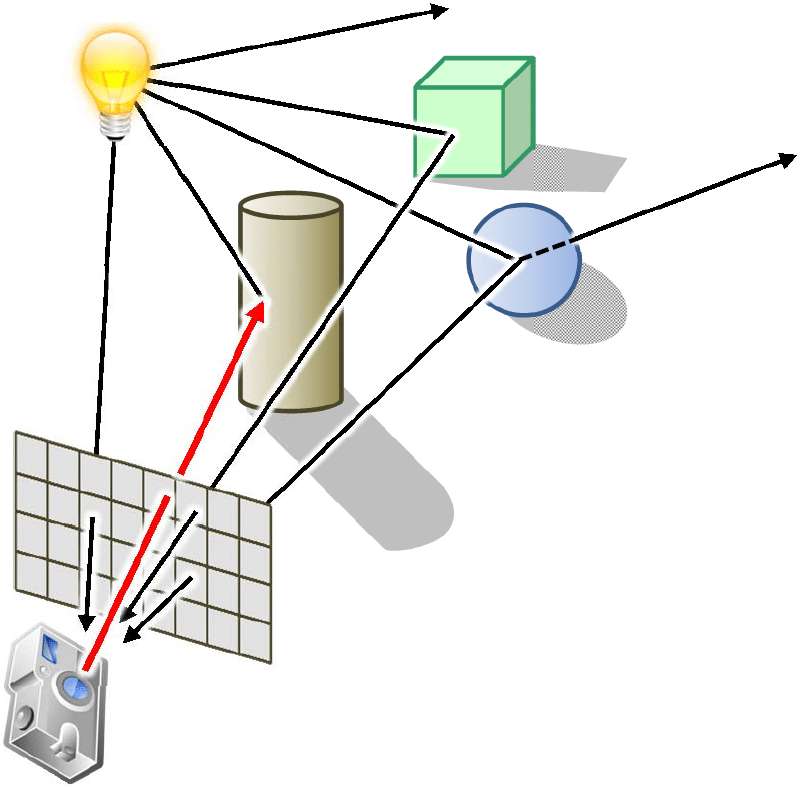
\includegraphics[width=\textwidth]{images/RayTracing.png}
    \caption{A schematic of ray tracing taken from computer graphics paper \cite{retzlaff2017physically}}
    \label{fig:18:raytracing}
\end{figure}
\section{Kolmogorov complexity and Kolmogorov $n$-width}
Recall that a reduced-order model (ROM) is an attempt to create a cheaper model that accurately approximates a more complex model. The inherent complexity of a model can be summarized by its \bt{Kolmogorov complexity}. In short, the Kolmogorov complexity is \q{the length of the shortest computer program that solves the problem.} It is the formalization of the introductory discussion of this section how cheaply we can store the information contained in the bit strings in Equations \eqref{eqn:18:simpleprogram} and \eqref{eqn:18:complexprogram}. 

The \bt{Kolmogorov $n$-width} of an object is a measure of how close an object is to its model approximation in lower dimensional space \askbjorn{Double check wording here}. Let $X$ be a normed linear space.
\begin{definition}{(Distance between point and subspace)}
Then we define the distance from a point $x \in X$ to an $n$-dimensional subspace $X_n \leq X$ as
\begin{align*}
    dist(x,X_n) := \inf_{y_n \in X_n} \|x - y_n\|_{X}.
\end{align*}
\end{definition}
This concept can be generalized to a subset $A \subseteq X$. It is defined as the largest distance from a point $x \in A$ to the subspace $X_n$. 
\begin{definition}{(Distance between subset and subspace)}
The distance between a subset $A \subseteq X$ and the $n$-dimensional subspace $X_n \leq X$ is defined as
\begin{align*}
    dist(A, X_n) := \sup_{x \in A} dist(x,X_n) = \sup_{x \in A} \left( \inf_{y_n \in X_n} \|x-y_n\|_{X} \right)
\end{align*}
\end{definition}
Finally, we are ready to define Kolmogorov $n$-width.
\begin{definition}{(Kolmogorov $n$-width)}
The Kolmogorov $n$-width of a set $A \subseteq X$ with respect to the normed space $X$\footnote{Note that the space $X$ and its associated norm $\|\cdot\|_{X}$ affects this computation.} is defined as
\begin{align*}
    d_{n}(A, X) &:= \inf_{\underset{dim(X_n)=n}{X_n \leq X}} dist(A,X_n) \\
        &= \inf_{\underset{dim(X_n)=n}{X_n \leq X}} \left[ \sup_{x \in A} \left( \inf_{y_n \in X_n} \|x - y_n\|_{X} \right)\right]
\end{align*}
\end{definition}
\askbjorn{Compare POD}

\chapter{Lecture 19}
\section{Landau rate}
Recall from last lecture that the Nyquist-Shannon sampling theorem tells us a minimal sampling rate necessary to recover a bandlimited signal. A generalization of the Nyquist sampling rate is the Landau rate. 
\cbeqn{Landau sampling rate}{
    \txt{If } \lambda\left(supp(\mathcal{F}(f))\right) = 2M > 0 \txt{ with } \lambda=\txt{Lebesgue measure}, \txt{ then } \label{eqn:18:nyquistsampling} \\
    f \txt{ is }  \txt{recovered by samples whose maximal step size is } \Delta t = \frac{1}{2M} \nonumber
}
\askbjorn{This seems to not be the right statement based on the paper by Landau. That paper seems to restrict attention to a finite union of compact intervals.}
The Landau sampling rate thus generalizes the Nyquist sampling theorem to (a) sets whose support in Fourier domain is disconnected and (b) to nonuniform grid sampling.

\askbjorn{Go through nonuniform sampling for homogenization}

\section{Kolmogorov $n$-width in context of POD}
Let us look at how Kolmogorov $n$-width relates to POD. Let $X=\R^2$ be our normed linear space and our set $A$ to be given by
\begin{align*}
    A = \{x=(x_1,x_2)\in \R^2 : x_2 = x_1 + sin(j x_1), j \in \mathbb{N}\}.
\end{align*}
This space is illustrated in Figure \ref{fig:19:A}. This figure shows us that $A$ is a sequence of sinusoidal perturbations of the identity. In our context, our norm is simply the Euclidean norm $\|\bs{x}\|_2^{2} = x_1^2 + x_2^2$. First, we note that $d_2(A,\R^2) = 0$ because $\R^2$ is the whole space and is a $2$-dimensional subspace of itself. What is $d_1(A,\R^2)$? One-dimensional subspaces are just lines passing through the origin, i.e. sets of the form $Y_{\alpha} = span\left[(\alpha, 1)^{T}\right]$ for some $\alpha$. 
\begin{figure}
    \centering
    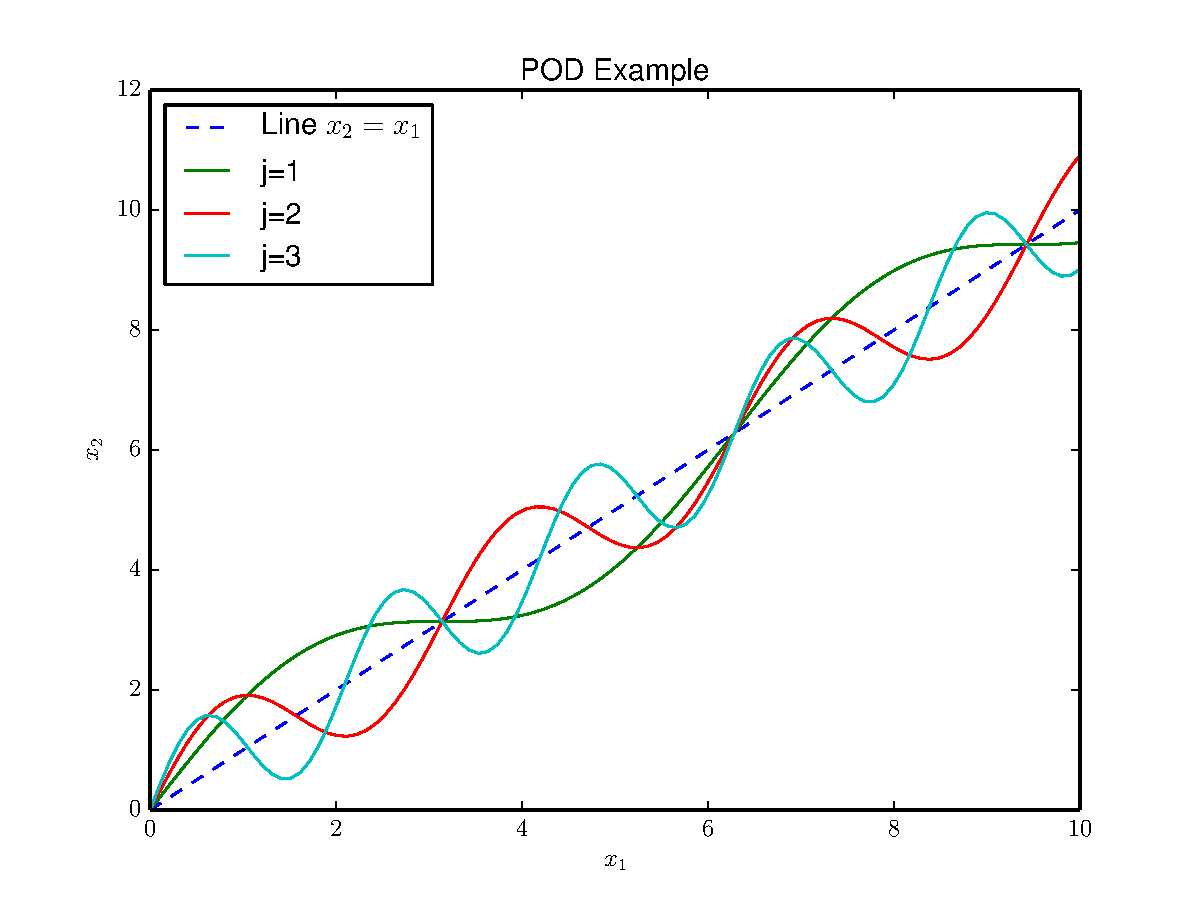
\includegraphics[width=\textwidth]{images/pod.pdf}
    \caption{Illustration of set $A$, which contains a sequence of sinusoidal perturbations of the identity.}
    \label{fig:19:A}
\end{figure}
Therefore, using the definition of Kolmogorov $1$-width, we can rewrite as
\begin{align} \label{eqn:19:kol1width}
d_1(A,\R^2) = \inf_{\alpha \in \R} \left[ \sup_{\bs{x} \in A} \left(\inf_{\bs{y} \in Y_{\alpha}} \|\bs{x}-\bs{y}\|\right)\right]
\end{align}
For $\bs{y} \in Y_{\alpha}$ and $\bs{x} \in A$, we have
\begin{align} \label{eqn:19:diff}
\|\bs{x} - \bs{y}\|^2 = (x_1 - y_1)^2 + (x_1 - \alpha y_1 + sin(j x_1))^2 := g(x_1,y_1).
\end{align}
The expression in Equation \eqref{eqn:19:kol1width} tells to first minimize over all values of $\bs{y}$ (that is, find $dist(\bs{x}, Y_{\alpha})$ first). Setting $\frac{\partial g}{\partial y_1} = 0$ and solving gives
\begin{align} \label{eqn:19:distY}
\frac{\partial g}{\partial y_1} = 0 &\Leftrightarrow y_1 = x_1 + \frac{\alpha}{1 + \alpha} sin(jx_1).
\end{align}
Plugging Equation \eqref{eqn:19:distY} into Equation \eqref{eqn:19:diff}, we arrive at
\begin{align} \label{eqn:19:inf}
\inf_{\bs{y} \in Y_{\alpha}} \|\bs{x} - \bs{y}\| = \sqrt{\frac{\alpha^2}{(1+\alpha)^2} sin^2(jx_1) + \left[ (1-\alpha)x_1 + \frac{\alpha^2 - \alpha - 1}{1+\alpha} sin(jx_1)\right]^2}
\end{align}
after taking the square root. Equation \eqref{eqn:19:kol1width} tells us that we now take a supremum over all $\bs{x} \in A$. We note that Equation \eqref{eqn:19:inf} shows us immediately that this supremum is infinite whenever $\alpha \neq 1$. The case when $\alpha=1$ reduces nicely to the expression $2^{-1/2} |sin(jx_1)|$ which takes maximal value $2^{-1/2}$. Thus we have
\begin{align}
    \sup_{\bs{x} \in A} \left( \inf_{\bs{y} \in Y_{\alpha}} \|\bs{x} - \bs{y}\|\right) = \begin{cases}
    \frac{1}{\sqrt{2}} & \alpha = 1 \\
    \infty & \alpha \neq 1
    \end{cases}
\end{align}
Our last step in Equation \eqref{eqn:19:kol1width} is take the infimum over all subspaces, i.e., over all slopes $\alpha$. This finally gives us that 
\begin{align} \label{eqn:19:kolfinal}
d_{1}(A,\R^2) = \inf_{\alpha \in \R} \left[ \sup_{\bs{x} \in A} \left( \inf_{\bs{y} \in Y_{\alpha}} \|\bs{x} - \bs{y} \| \right) \right] = \frac{1}{\sqrt{2}}
\end{align}
Note that this is consistent with our intuition that the best subspace should be the one defined by the identity. Furthermore, we have found the best rank-$1$ approximation of the set $A$ of interest; in this case the arg min of the expression for the Kolmogorov $1$-width is the space defined through the POD!

\askbjorn{Section regarding SVD}

\section{Dynamical Systems}
Consider the following dynamical system.
\begin{align} \label{eqn:19:dynamical}
\dot{\bs{x}}(t) &= \bs{A} \bs{x}(t) + B \bs{u}(t),  \hspace{5pt} \bs{x}(0) = \bs{0} \\
\bs{y}(t) &= \bs{C} \bs{x}(t) + \bs{D} \bs{u}(t)
\end{align}
where in practice, $dim(\bs{y})$, $dim(\bs{u}) \ll dim(\bs{x})$ and would like a ROM. We can rewrite
\begin{align} \label{eqn:19:hankel}
\bs{y}(t) = (S\bs{u})(t) := \int_{0}^{t} h(t-s) \bs{u}(s) ds
\end{align}
where
\begin{align} \label{eqn:19:hankelkernel}
h(t) = \bs{C} e^{\bs{A} t} \bs{B} + \bs{D} \delta(t).
\end{align}
$S$ is referred to as the \bt{Hankel operator} and its discretization the \bt{Hankel matrix}. Analysis can be done to see cases where the SVD of the Hankel matrix has low-rank structure and can thus lead to how well a ROM approximates the true solution. \askbjorn{There seems to be some inconsistent in my notation when I wrote this down. It is unclear to me whether Equation \eqref{eqn:19:dynamical} solves for vector-valued functions or scalar functions. When we say $dim(y) \ll dim(x)$, are we referring to the actual dimension of a vector or are we referring to the number of time samples necessary to obtain an accurate solution?}

\section{Model-Data Interaction}
We list a few types of data of interest below.
\begin{enumerate}
    \item Data for modeling \label{enu:19:model}
    \item Data for applying model \label{enu:19:applymodel}
    \item Data interaction when executing model \label{enu:19:exe}
        \begin{itemize}
            \item Data assimilation (meteorology, aerospace engineering)
            \item Digital twins (meteorology, manufacturing, even Amazon inventory modeling)
        \end{itemize}
\end{enumerate}
Item \ref{enu:19:model} is obvious for modeling in the context of data-driven models; it is simply the input to our model. For science-based modeling, data somewhat plays a background role. We typically have physical parameters that can be set and tested for inspiration, but largely, these are not updated dynamically in the course of the simulation, as is the goal with Item \ref{enu:19:exe}, data interaction. We note, however, that sometimes scientific models can be an intermediate step. Namely, scientific models can be used to create many examples of synthetic data that are then used to train data-driven models. When the data-driven model uses deep learning or some other machine learning technique, this process is often referred to as \bt{scientific machine learning}.

\chapter{Lecture 20}
\section{Model-Data Interaction}
We continue our discussion on model-data interaction. Consider the following ODE.
\begin{ceqn} \label{eqn:20:ode}
\frac{du}{dx} &= a(x) u(x) +  b(x) \\
u(0) &= u_0
\end{ceqn}
In the context of solving this ODE, our data are the parameters $a,b,u_0$. In the context of solving the inverse problem for this ODE, our data is the solution $Bu(x)$ where $B$ is an observation operator and $u$ is the solution to the ODE, and our output are the parameters $a,b,u_0$ (or some subset of these three, assuming that the others are known). The observation operator $B$ expresses the limits of our ability to observe the whole solution $u(x)$ in practice. For example, $Bu(x) = \{u(x_0),...,u(x_n)\}$ where $x_0,...,x_n$ live on a finite-element grid, recalling that FEM is able to find the exact values of the solution at the nodes.
\askbjorn{We seem to jump to interpolation of functions; should this be a subsection or its own section? Interpolation of functions seems to relate to the comment regarding observation operators}

\subsection{Interpolation in One Dimension}
In lieu of our previous comment, our goal is to find a continuous field given given data. This task is referred to as \bt{interpolation}. That is, given $\{f_j\}_{j=1}^{J}$ for grid points $\{x_1,..,x_J\}$ to approximate a model function $f(x)$. For simplicity, we assume that $f_j=f(x_j)$ is exactly for each $j$, which in the context of finite-element methods is the case (modulo floating point error). A few methods of interpolation are given below.

\begin{center}
\begin{enumerate}
    \item Polynomial interpolation \label{eqn:20:polyint}
    \item Piecewise polynomial interpolation \label{eqn:20:pcwpoly}
    \item Trigonometric interpolation \label{eqn:20:trigint}
    \item Kriging \label{eqn:20:krig}
    \item Other bases, e.g. wavelets \label{eqn:20:other}
\end{enumerate}
\end{center}
\tcr{figure out how to center this list}

\subsubsection{Polynomial interpolation}
Polynomial interpolation is based on the following theorem.
\begin{theorem}{(Polynomial interpolation)} \label{thm:20:polyint}
Let $\{(x_j,y_j)\}_{j=1}^{J}$ be a set of points with $x_j \neq x_k$ when $j \neq k$. Then there exists a unique polynomial $p$ of degree at most $J-1$ such that $p(x_j) = y_j$. 
\end{theorem}
The main advantage of polynomial interpolation is that the solution is analytic. However, the interpolation is extremely sensitive to perturbations and is thus, in general, not the best approach to interpolation. This sensitivity is referred to as \bt{Runge's phenomenon}. Consider the interval $I = [-1,1]$ and define the \bt{Runge function} $f : I \to \R$ by
\begin{align} \label{eqn:20:rungefnc}
f(x) = \frac{1}{1 + 25x^2}. 
\end{align}
Let $\mathcal{G}_{n} = \{x_0, x_1, ..., x_n\}$ with $x_j = -1 + \frac{2i}{n}$ be a uniform grid of $[-1,1]$ with $n+1$ points. Let $p_n$ be the interpolating polynomial given by Theorem \ref{thm:20:polyint}. Carl Runge showed the following result in 1901.
\begin{align} 
\lim_{n \to \infty} \|f - p_{n}\|_{L^{\infty}(I)} = \infty.
\end{align}
As $n \to \infty$, oscillations near the right endpoint get faster and larger, and this is what leads to this result. This is illustration in Figure \ref{fig:20:rungephen} which shows reasonable results up to degree $10$ and complete deterioritation of the approximation by degree $20$.
\begin{figure}
    \centering
    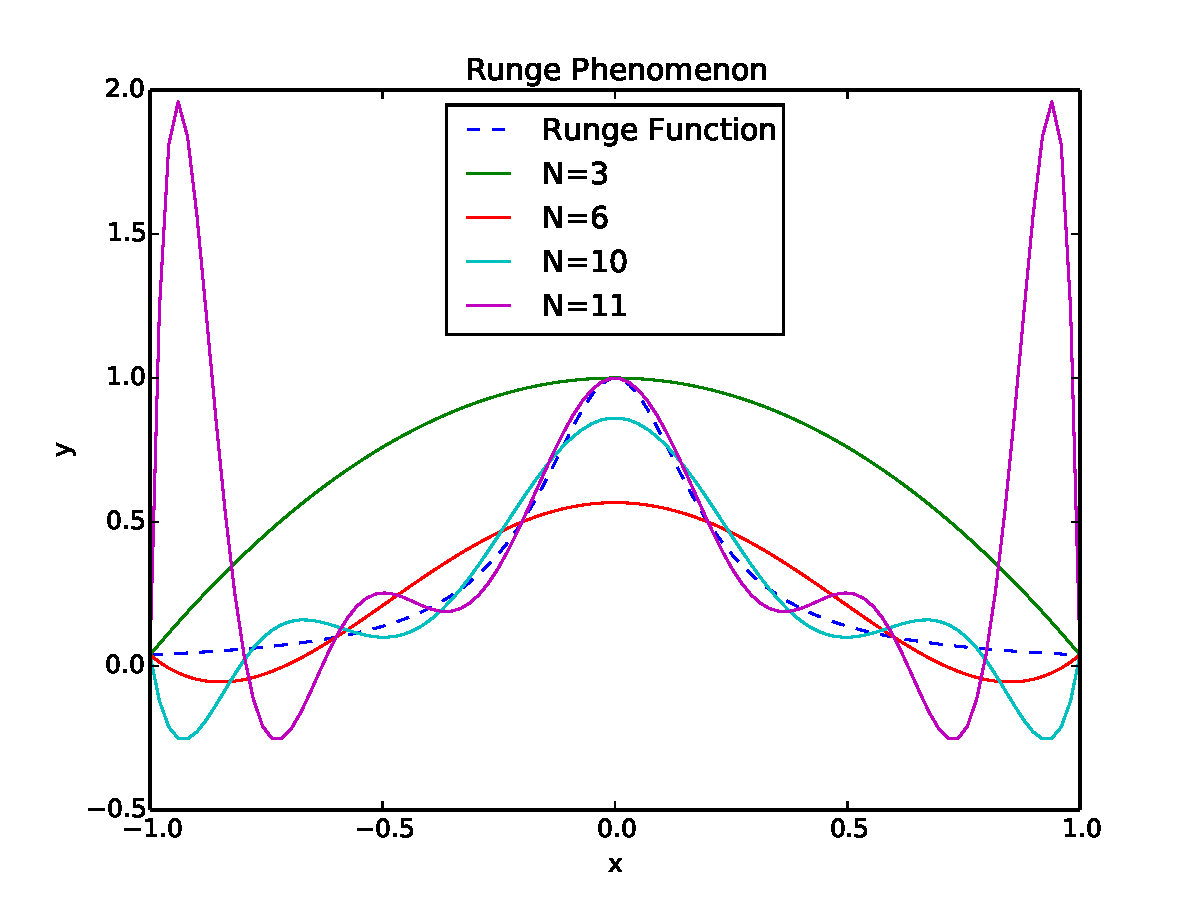
\includegraphics[width=\textwidth]{images/runge11.pdf}
    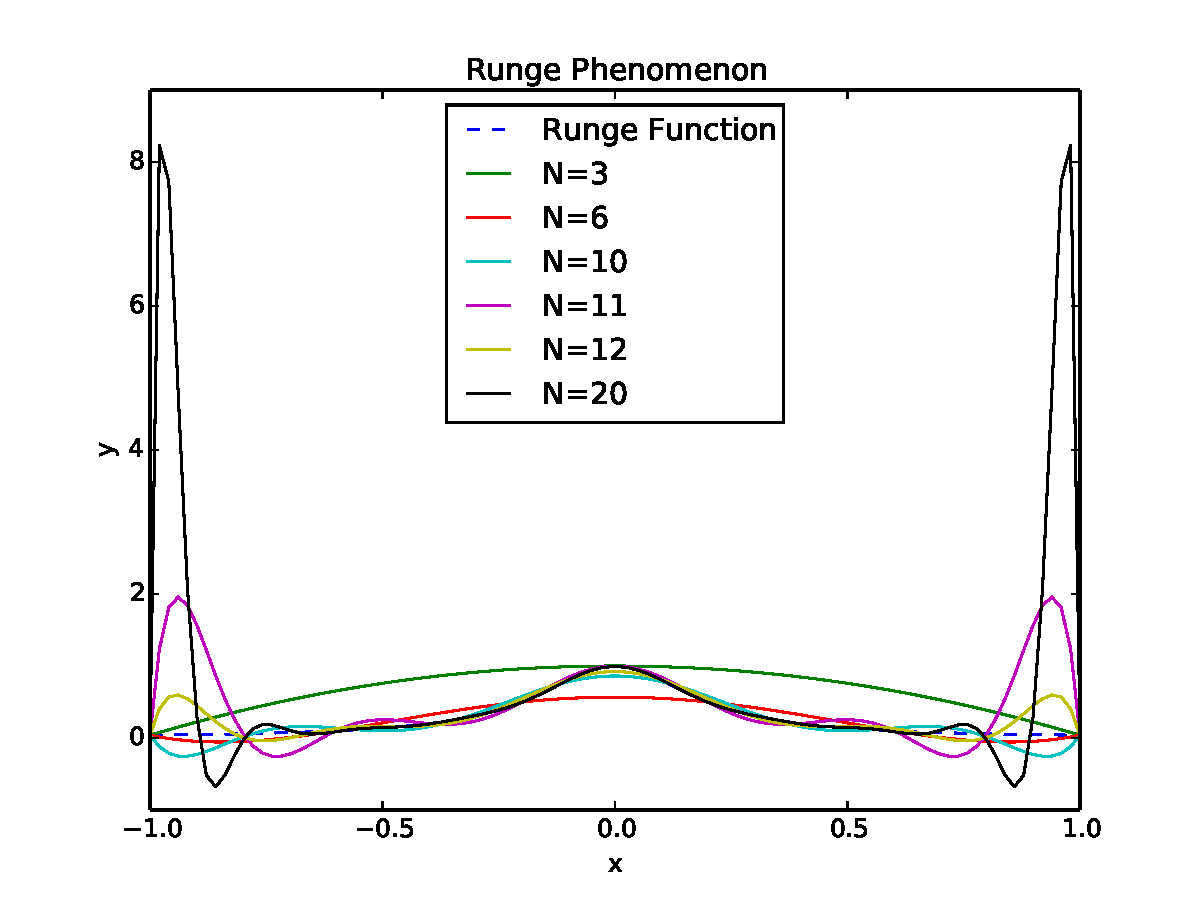
\includegraphics[width=\textwidth]{images/runge20.pdf}
    \caption{Increasing oscillation magnitude near the endpoints.}
    \label{fig:20:rungephen}
\end{figure}
Runge's phenomenon motivates the use of piecewise polynomial interpolation.

\subsubsection{Piecewise Polynomial Interpolation}
Instead of globally approximating our function $f$ by a polynomial, we approximate $f$ piecewise by multiple polynomials. The major advantage of this approach is that in contrast to global polynomial interpolation, piecewise polynomial interpolation is stable with respect to perturbations. The major disadvantages of this approach is that regularity at interfaces is lost and that a larger linear system of equations must be solved to extract coefficients for the polynomials. However, both of these issues can be worked around to some degree. B-splines are a type of piecewise polynomial which allows for control of the smoothness at the interfaces! Furthermore, the linear systems needed to obtain the coefficients can, in certain contexts, be precomputed. \askbjorn{Come up with an example of this; note also that this is a question I posed during class, so the precomputation might not be as strong as I'm interpreting and \bjorn and I had a miscommunication here...it seems to me that the cost of the linear system is essentially negligible since this system could be solved up to say order $30$, which is basically overkill as it is}. 

\subsubsection{Trigonometric Interpolation}
Trigonometric interpolation needs $\{x_j\}$ to be uniformly spaced for efficiency. Constraints to obtain the coefficients are often obtained with either (a) direct formulae or (b) an optimization method such as gradient descent or the Newton-Raphson method.

\subsubsection{Kriging}
We will return to this topic later.

\subsubsection{Other methods}
\askbjorn{Not exactly sure I understand the motivation for the equation I have written down in the iPad.}

\subsection{Interpolation in Higher Dimensions}


\chapter{Lecture 21}
Regarding our discussion of interpolation from the previous lecture, what if instead of observing our ground truth function $f$, we instead observe $f + \eta$ with noise $\eta$? 
\section{Cross-validation}
Cross-validation is a class of techniques used to assess the generalizability of a model to different data sets. The central idea behind cross-validation is to interpolate a target function $f$ on a proper subset of its domain and then check the error on all the data points that were not considered during the initial interpolation. If this error is low, we may be more confident in our interpolation's generalizability.

\subsection{Linear regression with leave-$p$-out cross-validation}
We motivate this process with an example with linear regression. We are given observations $Y=\{\bs{y}_1,...,\bs{y}_J\} \subseteq \R^{d}$ with
\begin{align}
    \bs{y}_j = \bs{f}_j + \bs{\eta}_j
\end{align}
and $\bs{f}_j \approx \bs{f}(\bs{x}_j)$ for target $\bs{f}$ and noise $\bs{\eta}_j$. In linear regression, we wish to solve for $\bs{\alpha}$ and $\bs{\beta}$ such that
\begin{ceqn} \label{eqn:21:linreg}
    L = \sum_{j=1}^{J} \left(\bs{y}_j - \hat{\bs{y}}_j\right)^2 \\
    \hat{\bs{y}}_{j} = \bs{\alpha} + \bs{\beta} \cdot \bs{x}_j
\end{ceqn}
is minimized. Our approach in this example will be \bt{leave-$p$-out} cross-validation. We first select a valid set $V = \{\bs{y}_{j_1},...,\bs{y}_{j_p}\}$ and a training set $T = Y \setminus V$. We then solve the auxiliary problem to find $\bs{\alpha}_{0}$ and $\bs{\beta}_{0}$ such that
\begin{align} \label{eqn:21:linregaux}
L_{T} &:= \sum_{j \in T} \left( \bs{y}_{j} - \hat{\bs{y}}_{j} \right)^2 
\end{align}
is minimized. The validation error is then defined by
\begin{ceqn} \label{eqn:21:linregval}
    L_{V} &:= \sum_{j \in V} \left( \bs{y}_j - \hat{\bs{y}_{j,T}} \right)^2 \\
    \hat{\bs{y}}_{j,T} &:= \bs{\alpha}_0 + \bs{\beta}_0 \cdot \bs{x}_{j}.
\end{ceqn}
Finally, we define the total cross-validation error as
\begin{align} \label{eqn:21:crossval}
    L_{cross} := \sum_{V \in \mathcal{V}} L_{V}
\end{align}
where
\begin{align} \label{eqn:21:v}
\mathcal{V} := \{ V \subseteq Y : |V|=p \}.
\end{align}
Note that Equations \eqref{eqn:21:crossval} and \eqref{eqn:21:v} express that we exhaustively check validation sets of size $p$. This may be untenable for large $J$ and $p$ since 
\begin{align*}
    |\mathcal{V}| = \binom{J}{p}
\end{align*}
grows very quickly with $J$ as long as $p$ is reasonably far away from $0$ and from $J$.
In the case of linear regression, it can be shown that the expected cross-validation loss is given by
\begin{align} \label{eqn:21:lossest}
\EE{L} = \frac{n-p-1}{n+p+1} \EE{L_{cross}}.
\end{align}
Equation \eqref{eqn:21:lossest} can be used to determine whether we are overfitting our data when using linear regression. A figure showing this phenomenon can be seen below.
\begin{figure}
    \centering
    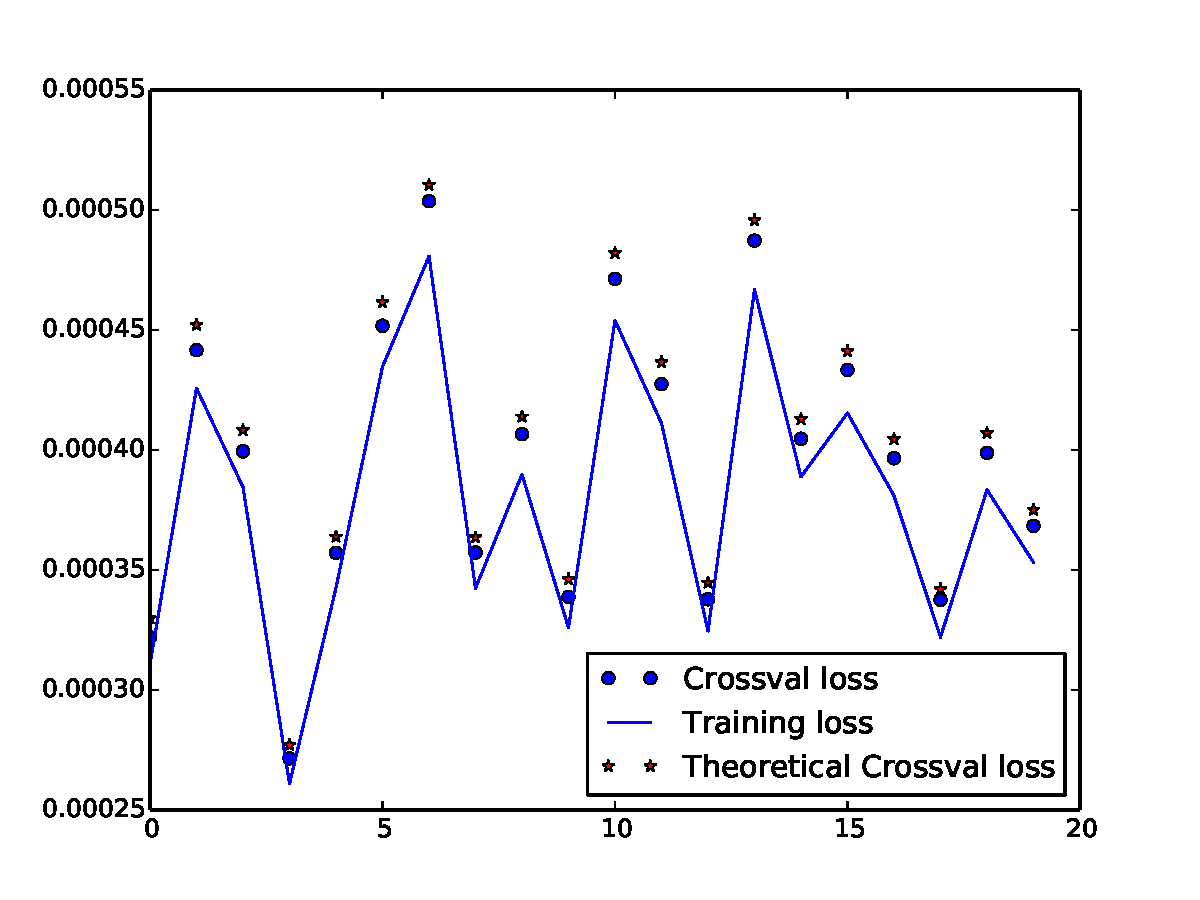
\includegraphics[width=\textwidth]{images/linreg-crossval.pdf}
    \caption{Code to produce this figure can be found \href{https://github.com/tmasthay/MathModeling/tree/main/lectures/lecture21}{here}.}
    \label{fig:21:crossval}
\end{figure}

\section{Choice of norms}
Say we have observations $\bs{f} = (f(\bs{x}_1),...,f(\bs{x}_n))^{T}$. Note that the optimization outlined in Equation \eqref{eqn:21:linregaux} is possibly the most common for approximation, i.e., least-squares or $L^2$ minimization.
However, we do not need to minimize with respect to $L^2$ for approximation, and in some contexts, we may be better off using a different norm. 

In general, $L^2$ is (a) a compromise between $L^{\infty}$ and $L^{1}$ minimization, (b) has ``good statistical properties'' in some sense, and (c) lends itself to efficient numerical algorithms. $L^1$ minimization is typically more robust than $L^2$ with respect to noise. Intuitively, this is because the squaring of the difference exacerbates the effect of an outlier. Finally, $L^{\infty}$ is very sensitive to noise because it exacerbates this outlier issue even more than $L^2$. $L^{\infty}$ typically finds its application for softwares such as numerical libraries for worst-case bounds on the error of approximations for evaluations such as Taylor series. \askbjorn{Draw informative pictures to outline here}. There are obviously many other norms to optimize with, but this is beyond the scope of our discussion.

As far as computational methods, $L^2$ optimization is usually solved with the normal equations. These can be solved without matrix decomposition or with the QR decomposition or SVD. These decompositions are more robust but more expensive. $L^1,L^{\infty}$ optimization are typically solved through linear programming. The general form for linear programming is given below.
\begin{ceqn}
    &\min_{\bs{x} \in \mathbb{R}^{n}} \bs{c} \cdot \bs{x} \\
    &\textup{subject to } \bs{A} \bs{x} - \bs{b} \leq \bs{0}, \bs{x} \geq \bs{0} 
\end{ceqn}
\chapter{Lecture 22}
\chapter{Lecture 23}
\chapter{Lecture 24}
\chapter{Lecture 25}

%%%%%%%%%%%%%%%%%%%%%% appendix.tex %%%%%%%%%%%%%%%%%%%%%%%%%%%%%%%%%
%
% sample appendix
%
% Use this file as a template for your own input.
%
%%%%%%%%%%%%%%%%%%%%%%%% Springer-Verlag %%%%%%%%%%%%%%%%%%%%%%%%%%

\appendix
\motto{All's well that ends well}
\chapter{Chapter Heading}
\label{introA} % Always give a unique label
% use \chaptermark{}
% to alter or adjust the chapter heading in the running head

Use the template \emph{appendix.tex} together with the Springer document class SVMono (monograph-type books) or SVMult (edited books) to style appendix of your book.


\section{Section Heading}
\label{sec:A1}
% Always give a unique label
% and use \ref{<label>} for cross-references
% and \cite{<label>} for bibliographic references
% use \sectionmark{}
% to alter or adjust the section heading in the running head
Instead of simply listing headings of different levels we recommend to let every heading be followed by at least a short passage of text. Furtheron please use the \LaTeX\ automatism for all your cross-references and citations.


\subsection{Subsection Heading}
\label{sec:A2}
Instead of simply listing headings of different levels we recommend to let every heading be followed by at least a short passage of text. Furtheron please use the \LaTeX\ automatism for all your cross-references and citations as has already been described in Sect.~\ref{sec:A1}.

For multiline equations we recommend to use the \verb|eqnarray| environment.
\begin{eqnarray}
\vec{a}\times\vec{b}=\vec{c} \nonumber\\
\vec{a}\times\vec{b}=\vec{c}
\label{eq:A01}
\end{eqnarray}

\subsubsection{Subsubsection Heading}
Instead of simply listing headings of different levels we recommend to let every heading be followed by at least a short passage of text. Furtheron please use the \LaTeX\ automatism for all your cross-references and citations as has already been described in Sect.~\ref{sec:A2}.

Please note that the first line of text that follows a heading is not indented, whereas the first lines of all subsequent paragraphs are.

% For figures use
%
\begin{figure}[t]
\sidecaption[t]
%\centering
% Use the relevant command for your figure-insertion program
% to insert the figure file.
% For example, with the option graphics use
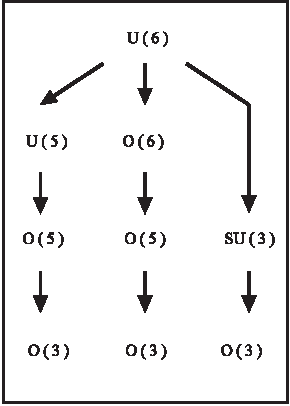
\includegraphics[scale=.65]{figure}
%
% If not, use
%\picplace{5cm}{2cm} % Give the correct figure height and width in cm
%
\caption{Please write your figure caption here}
\label{fig:A1}       % Give a unique label
\end{figure}

% For tables use
%
\begin{table}
\caption{Please write your table caption here}
\label{tab:A1}       % Give a unique label
%
% For LaTeX tables use
%
\begin{tabular}{p{2cm}p{2.4cm}p{2cm}p{4.9cm}}
\hline\noalign{\smallskip}
Classes & Subclass & Length & Action Mechanism  \\
\noalign{\smallskip}\hline\noalign{\smallskip}
Translation & mRNA$^a$  & 22 (19--25) & Translation repression, mRNA cleavage\\
Translation & mRNA cleavage & 21 & mRNA cleavage\\
Translation & mRNA  & 21--22 & mRNA cleavage\\
Translation & mRNA  & 24--26 & Histone and DNA Modification\\
\noalign{\smallskip}\hline\noalign{\smallskip}
\end{tabular}
$^a$ Table foot note (with superscript)
\end{table}
%


\backmatter%%%%%%%%%%%%%%%%%%%%%%%%%%%%%%%%%%%%%%%%%%%%%%%%%%%%%%%
%%%%%%%%%%%%%%%%%%%%%%%acronym.tex%%%%%%%%%%%%%%%%%%%%%%%%%%%%%%%%%%%%%%%%%
% sample list of acronyms
%
% Use this file as a template for your own input.
%
%%%%%%%%%%%%%%%%%%%%%%%% Springer %%%%%%%%%%%%%%%%%%%%%%%%%%

\Extrachap{Glossary}


Use the template \emph{glossary.tex} together with the Springer document class SVMono (monograph-type books) or SVMult (edited books) to style your glossary\index{glossary} in the Springer layout.


\runinhead{glossary term} Write here the description of the glossary term. Write here the description of the glossary term. Write here the description of the glossary term.

\runinhead{glossary term} Write here the description of the glossary term. Write here the description of the glossary term. Write here the description of the glossary term.

\runinhead{glossary term} Write here the description of the glossary term. Write here the description of the glossary term. Write here the description of the glossary term.

\runinhead{glossary term} Write here the description of the glossary term. Write here the description of the glossary term. Write here the description of the glossary term.

\runinhead{glossary term} Write here the description of the glossary term. Write here the description of the glossary term. Write here the description of the glossary term.
%
\Extrachap{Solutions}

\section*{Problems of Chapter~\ref{intro}}

\begin{sol}{prob1}
The solution\index{problems}\index{solutions} is revealed here.
\end{sol}


\begin{sol}{prob2}
\textbf{Problem Heading}\\
(a) The solution of first part is revealed here.\\
(b) The solution of second part is revealed here.
\end{sol}


\printindex

\bibliography{author/refs}
%%%%%%%%%%%%%%%%%%%%%%%%%%%%%%%%%%%%%%%%%%%%%%%%%%%%%%%%%%%%%%%%%%%%%%

\end{document}





